% ============================================================
% Manuscript formatted for PRX Quantum (REVTeX 4.2, APS).
% Section, subsection, figure, and table structure mirror the JMLR paper
%   Hashimoto, Hafid, Ikeda & Kadri, "Spectral Truncation Kernels:
%   Noncommutativity in C*-algebraic Kernel Machines" (arXiv:2405.17823),
% rephrased correspondingly into the QAOA angle-search setting and kept
% consistent with arXiv:2606.22630: ten numbered sections (Introduction,
% Preliminaries, the proposed prior, a budget bound, the angle search, a
% combined-model extension, applications, numerical results, generalizations,
% and conclusion & discussion), with seven main-body figures and two
% main-body tables, as in that paper.  Content (references, numbers, claims)
% is unchanged from the author's manuscript; only the scaffolding follows the
% mirrored layout.
%
% Figures, tables, and numeric results are regenerated by:
%   cd submission/code
%   pip install .
%   ostqaoa-reproduce --output-dir . --depth 3 --budget 24 --rank 4 --commutator-weight 4.0
%   python multiseed_robustness.py          % per-seed robustness CSV
%   python make_jmlr_mirror_artifacts.py    % the four added display items + Table I
% ============================================================
\documentclass[aps,prxquantum,reprint,amsmath,amssymb,floatfix,nofootinbib,superscriptaddress,longbibliography]{revtex4-2}

\usepackage{amsthm}
\usepackage{graphicx}
\graphicspath{{code/figures/}}
\usepackage{booktabs}
\usepackage{bm}
\usepackage[hidelinks]{hyperref}
\usepackage{cleveref}

\newtheorem{theorem}{Theorem}
\newtheorem{lemma}{Lemma}
\newtheorem{corollary}{Corollary}
\newtheorem{definition}{Definition}
\newtheorem{proposition}{Proposition}
\newtheorem{assumption}{Assumption}
\theoremstyle{remark}
\newtheorem{remark}{Remark}

% cleveref names for the theorem-like environments added for the
% statistical-theory section (Sec.~\ref{sec:stattheory}).
\crefname{theorem}{Theorem}{Theorems}
\Crefname{theorem}{Theorem}{Theorems}
\crefname{lemma}{Lemma}{Lemmas}
\Crefname{lemma}{Lemma}{Lemmas}
\crefname{corollary}{Corollary}{Corollaries}
\Crefname{corollary}{Corollary}{Corollaries}

\newcommand{\QAOA}{\textnormal{\textsc{QAOA}}}
\newcommand{\OSTQAOA}{\textnormal{\textsc{OST-QAOA}}}
\newcommand{\TQA}{\textnormal{\textsc{TQA}}}
\newcommand{\calG}{\mathcal{G}}
\newcommand{\calL}{\mathcal{L}}
\newcommand{\calO}{\mathcal{O}}
\newcommand{\calA}{\mathcal{A}}
\newcommand{\calB}{\mathcal{B}}
\newcommand{\calC}{\mathcal{C}}
\newcommand{\bbR}{\mathbb{R}}
\newcommand{\cmark}{\ensuremath{\checkmark}}
\newcommand{\xmark}{\ensuremath{\times}}

\begin{document}

\title{Operator-Spectral Truncated Priors for Query-Efficient QAOA Parameter Search}

\author{Molena Huynh}
\email{molena.huynh@jmp.com}
\affiliation{North Carolina State University, Raleigh, North Carolina 27695, USA}

\date{\today}

\begin{abstract}
From the keyboard a quantum computer is a stochastic device: the Born rule returns
one bitstring per run, so tuning a variational circuit is stochastic optimization
of an objective---the expectation \(\langle H_C\rangle\)---that can only be
\emph{estimated}, and the scarce resource is the number of such estimates.
We introduce \OSTQAOA{}, a method that treats angle tuning as Bayesian search and
works in operator space rather than raw parameter-vector space to overcome the true
bottleneck of low-depth \QAOA{}:
the objective queries available to tune angles on each new graph.  It maps each
graph to a truncated symmetric operator on the \(2p\)-dimensional angle space,
built from two noncommuting graph-derived generators, and converts its low-rank
spectral decomposition into ranked collective search directions for a
deterministic, auditable query policy.  We prove the prior covariance is positive
definite, truncation is Loewner-monotone, the construction reduces to
per-angle coordinate refinement in its commutative limit, and truncation caps the
effective search dimension; a validated scaling argument links truncation to
query cost.  On exact-statevector MaxCut over four graph families, a ten-seed
study (\(160\) paired held-out instances) beats a budget-matched \TQA{} baseline
by \(+0.104\pm0.012\) mean approximation ratio (\(153/160\) wins) and reaches
\(98\%\) of the best ratio in \(10.7\) queries against \(24.6\), a \(2.3\times\)
reduction; at the reference point (\(p{=}3\), rank \(4\), weight \(4.0\)) it
reaches \(0.818\pm0.019\), \(+0.110\) over baseline (sign-test \(p<10^{-4}\)).  A
truncation sweep shows the predicted interior optimum, and an ablation localizes
the gain to noncommutative directions (\(-0.009\) when restricted to diagonal
ones).  We accompany these findings with a statistical theory of the truncated
prior---Eckart--Young--Mirsky optimality, posterior contraction with an interior
optimal rank, and an \(d_{\mathrm{eff}}\)-controlled query-complexity gain---and
ship the method as the installable package \texttt{specops-ostqaoa}, whose single
command \texttt{ostqaoa-reproduce} regenerates every figure, table, and query
trace from tunable parameters.  \OSTQAOA{} is thus a rigorous, reproducible
operator-valued prior that makes query efficiency, not sampling volume, the
lever for near-term variational search on graphs.
\end{abstract}

\maketitle

% ============================================================
\section{Introduction}
% ============================================================

Statistics is under-rated in, and structural to, quantum computing.  From the
keyboard a quantum computer is a stochastic device interrogated only by sampling:
the Born rule returns one bitstring per run, so the value a variational algorithm
optimizes---the expectation \(\langle H_C\rangle\)---is never observed directly but
\emph{estimated}, with a variance, a confidence interval, and a sample-complexity
cost.  Tuning the circuit is therefore stochastic optimization over an objective
one can only estimate, and the scarce resource is the number of estimates the
policy is allowed to spend.  This paper takes that statistical reading literally:
it treats angle tuning as Bayesian search under a graph-conditioned prior, so that
the truncated operator we build is a probabilistic surrogate for the expensive
quantum objective whose spectrum \emph{is} the ranked search geometry, and query
efficiency is a matter of injecting the right prior structure rather than of
sampling more.

Many combinatorial graph-optimization problems---including instances arising in
biomedical settings such as pathway-subset selection and patient-similarity
partitioning---can be cast as graph objectives, with MaxCut a canonical example
of the broad class of \(\mathrm{NP}\)-hard problems admitting Ising
formulations~\cite{karp1972,lucas2014}, classically approached by the
Goemans--Williamson semidefinite relaxation~\cite{goemans1995}.  \QAOA{}~\cite{farhi2014,farhi2014bounded}
provides a variational quantum template for them, with MaxCut its canonical
benchmark~\cite{crooks2018,wurtz2021,wurtz2021fixed} and one instance of the broader
variational-quantum-algorithm paradigm~\cite{cerezo2021}.
The alternating-operator structure generalizes beyond the original
mixer~\cite{hadfield2019}, admits a fermionic analysis on MaxCut~\cite{wang2018fermionic},
and is itself computationally universal~\cite{lloyd2018}; see~\cite{blekos2024}
for a survey.  In the noisy
intermediate-scale regime~\cite{preskill2018}, however, practical use is gated
less by the circuit
than by the \emph{classical policy} that decides how to spend a small budget of
expensive objective evaluations on each new instance---a classical optimization
that is itself \(\mathrm{NP}\)-hard in general~\cite{bittel2021} and sensitive to
the choice of optimizer on noisy
objectives~\cite{lavrijsen2020,pellowjarman2021,larkin2022}.  A good warm-start point
alone is not enough: under a fixed query budget the optimizer also needs to know
\emph{which angle directions} deserve exploration.

A large body of work shows that good QAOA angles transfer across instances.
Objective values concentrate for fixed parameters on typical
instances~\cite{brandao2018,zhou2020}, optimal parameters concentrate with system
size~\cite{akshay2021}, and parameters trained on one graph transfer to
others~\cite{galda2021,shaydulin2023transfer}, an ingredient even in recent
demonstrations of scaling advantage on hardware~\cite{shaydulin2024,harrigan2021,pagano2020}.
Trotterized--annealing (\TQA{})
schedules supply strong instance-independent initializations~\cite{sack2021},
reflecting the adiabatic and quantum-annealing roots of the
ansatz~\cite{farhi2001adiabatic,kadowaki1998}.  Related warm-start and
learned-initialization strategies start the optimizer from a relaxation
solution~\cite{egger2021warmstart}, a graph-neural-network
prediction~\cite{jain2022gnn}, or a meta-learned
policy~\cite{khairy2020}.
These results motivate \emph{transferring structure} between graphs; what they do
not specify is a budgeted search geometry---the directions, and their relative
scales, along which a few queries should be spent once a warm start is in hand.

The central idea of this work is to learn and search in \emph{operator space}
rather than only in parameter-vector space.  For a graph \(G\), \OSTQAOA{}
constructs two \(2p\times2p\) symmetric operators from the graph Laplacian
spectrum, degree moments, and topology features.  Their noncommuting product
defines a commutator energy, and a truncated spectral decomposition of the
resulting angle operator gives a low-rank covariance.  The covariance is not used
as a passive uncertainty estimate; it becomes the ranked list of search
directions evaluated by a deterministic query policy that can be audited line by
line.  This is the accelerate-science-with-a-surrogate move made concrete for a
quantum objective: rather than emulate a scalar output, the prior emulates the
\emph{local geometry} of an expensive stochastic simulator---the graph's QAOA
landscape---and does so \emph{interpretably}, because the science is built in.  The
generators \(\calA_G,\calB_G\) encode mechanistic graph descriptors (Laplacian
spectrum, degree moments, topology), so the retained eigendirections are named,
graph-derived collective moves rather than opaque learned features, and the
truncation rank makes the surrogate's capacity explicit.  Integrating that
domain structure is what lets the prior learn a usable search geometry from a
handful of noisy objective queries and act on it with calibrated confidence.

This is motivated by, but distinct from, the spectral-truncation kernel
framework of Hashimoto \emph{et al.}~\cite{hashimoto2024spectral}, in which
truncation of positive-definite \(C^*\)-algebraic kernels controls
noncommutativity and trades representation power against model complexity.  Here
the output is not a supervised vector-valued regression kernel.  It is a
graph-conditioned prior over \QAOA{} angles, together with a deterministic
objective-query policy.  We adopt the design idea---finite-rank noncommutativity
as a tractable way to encode interaction---and ask what it buys in the operational
currency that limits near-term QAOA, namely the number of objective queries.
The same kernel/feature-space viewpoint underlies quantum machine
learning~\cite{schuld2019feature}, and using machine-learned
structure to guide combinatorial search is a broader
theme~\cite{bengio2021}; the prospect of a quantum advantage from low-depth
QAOA~\cite{farhi2016supremacy} makes the query cost of tuning it the decisive
near-term quantity.

\paragraph{Scope.}  To keep every reported number exactly reproducible on a CPU,
all experiments use small exact statevectors (\(n\le10\)) and brute-force MaxCut
optima on standard synthetic graph families.  This is a methods study of a search
policy, not a claim of hardware-scale or domain (e.g.\ biomedical) deployment;
\cref{sec:conclusion} states the limitations and the path to scale.

\paragraph{Contributions.}  The two program themes above---that statistics is
structural to quantum computing (Born-rule sampling makes the objective an
estimand, so tuning is estimation-and-inference) and that an interpretable
Bayesian surrogate can accelerate an expensive quantum computation---are made
concrete here in four contributions.
\begin{enumerate}
\item \textbf{A new operator-valued prior and search algorithm.}  \OSTQAOA{}
constructs a truncated, noncommuting operator on QAOA angle space---rather than a
scalar graph feature or a diagonal uncertainty vector---from two graph-derived
generators \(\calA_G,\calB_G\) that do not commute, spectrally truncates it to a
rank-\(n\) covariance (\cref{eq:operator,def:trunc}), and turns its ranked
eigendirections into a deterministic, auditable objective-query policy
(\cref{sec:search}).  The off-diagonal geometry is used operationally: the policy
probes the \emph{collective} eigendirections of \(\Sigma_G\), not the raw angle
coordinates.
\item \textbf{A rigorous statistical theory of the truncated prior.}  Reading the
truncated operator as a Gaussian-process prior over the angle objective, we prove
its covariance is positive definite (\cref{prop:pd}) and Loewner-monotone in the
rank (\cref{prop:mono}), reduces exactly to the commutative diagonal prior in the
\(n\to1\) limit (\cref{prop:limit}), and caps the effective dimension
\(d_{\mathrm{eff}}(n)\) (\cref{prop:deff}).  On top of these we establish four
theorems: truncation error is the sharp Eckart--Young--Mirsky tail mass
(\cref{thm:eym}); the GP posterior contracts at a rate set by the retained
spectrum with an interior optimal rank \(r^{\star}\) (\cref{thm:contraction}); the
surrogate's excess risk is controlled by the retained effective dimension, not by
the ambient angle dimension (\cref{thm:rkhs}); and reaching \(\varepsilon\)-accuracy
costs a factor \(d_{\mathrm{eff}}/2p\) fewer quantum objective queries than an
uninformative prior (\cref{thm:query}).
\item \textbf{Empirical query-efficiency gains with real headline numbers.}  On
exact-statevector MaxCut over four graph families, \OSTQAOA{} reaches
\(0.818\pm0.019\) mean approximation ratio at the reference point, \(+0.110\) over
budget-matched \TQA{}+coordinate (\(16/16\) wins, sign-test \(p<10^{-4}\);
\cref{tab:headline}), and across ten seeds (\(160\) paired instances) improves by
\(+0.104\pm0.012\), positive on every seed with \(153/160\) instance wins and a
\(2.3\times\) query reduction (\cref{fig:robust}).  A truncation sweep exhibits
the predicted interior optimum \(n^{\star}{=}4\) (\cref{fig:sweep}), and an
ablation localizes the gain to the noncommuting off-diagonal directions
(\(-0.009\) mean ratio when restricted to the diagonal; \cref{sec:synthetic}).
The operational query-budget scaling of \cref{rem:query} is stated as an explicit
heuristic under a coverage assumption and tested, not asserted.
\item \textbf{A reproducible, installable artifact.}  The method ships as the pip
package \texttt{specops-ostqaoa}, whose single console command
\texttt{ostqaoa-reproduce} regenerates every figure, table, CSV, and query trace
from one seed---and re-derives the headline advantage across ten seeds---while a
Python API exposes depth, budget, rank, commutator weight, seed, and graph family
for retuning every experimental parameter.
\end{enumerate}

This work continues a single-author program on spectral truncation of
operators for query-efficient quantum optimization.  Earlier entries develop
graph-conditioned trust regions for query-efficient and uncertainty-calibrated
\QAOA{}~\cite{huynh2026gctr,huynh2026gctrcalpro}, the
measurement cost of warm-started low-depth \QAOA{} and certified query
budgets~\cite{huynh2026meascost,huynh2026certqb}, and topology-conditioned
parameter transfer for budgeted graph
optimization~\cite{huynh2026paramxferB}.
The common thread
is to fix a small objective-query budget and decide, from graph structure, where
those queries are spent.  Here we move that decision from a scalar trust region
or a transferred point into a truncated, noncommuting operator on the full angle
space, so the search geometry itself is conditioned on the graph and the
truncation rank sets the number of collective directions probed.

% ============================================================
\section{Preliminaries}
\label{sec:prelim}
% ============================================================

\subsection{QAOA and the angle-space objective}
\label{sec:qaoa}

Let \(G=(V,E)\) be an undirected graph with \(n=|V|\).  The MaxCut Hamiltonian is
\begin{equation}
    H_C(G)=\sum_{(i,j)\in E}\frac{1-Z_iZ_j}{2}.
\end{equation}
At depth \(p\), the QAOA parameter vector is
\(\theta=(\gamma_1,\ldots,\gamma_p,\beta_1,\ldots,\beta_p)\in[0,\pi]^{2p}\),
and with mixer \(H_M=\sum_i X_i\) the state and objective are
\begin{align}
    |\psi_G(\theta)\rangle &=
    \prod_{\ell=1}^{p}e^{-i\beta_\ell H_M}e^{-i\gamma_\ell H_C(G)}
    |+\rangle^{\otimes n}, \\
    f_G(\theta)&=\langle\psi_G(\theta)|H_C(G)|\psi_G(\theta)\rangle .
\end{align}
We report the approximation ratio \(r_G(\theta)=f_G(\theta)/C_G^\star\), where
\(C_G^\star\) is computed exactly by brute force for the small audit graphs used
here.  An algorithm receives a fixed query budget \(Q\), where one query is one
exact evaluation of \(f_G(\theta)\); each method is measured by the best ratio
found within the same \(Q\).  This query model is deliberately simple: it
isolates the angle-search policy from finite-shot readout and hardware noise,
which \cref{sec:conclusion} discusses as the next experimental layer.  The
\(2p\)-dimensional angle space \([0,\pi]^{2p}\) plays the role that the data
function domain plays for an operator-valued kernel: it is the space on which our
operators act.

\subsection{Spectral truncation on the angle operator}
\label{sec:trunc}

Spectral truncation replaces an operator by the part of its spectrum carried by
its leading directions.  Given a symmetric operator \(\calO\) on angle space with
eigendecomposition \(\calO=U\Lambda U^{\mathsf T}\), retaining the \(r\) leading
eigenpairs and clipping their eigenvalues to be nonnegative yields a rank-\(r\)
positive-semidefinite operator.  In the \(C^*\)-algebraic setting this is the
truncation operation controlled by a parameter that interpolates between
commutative and noncommutative products~\cite{hashimoto2024spectral}; here it is
the truncation of the angle operator that we construct in \cref{sec:method}.

\begin{definition}[Spectral truncation on angle space]
\label{def:trunc}
Let \(\calO_G=U\Lambda U^{\mathsf T}\).  For truncation rank \(r\), define
\(\calO_{G,r}=U_r\Lambda_rU_r^{\mathsf T}\), where \(U_r\) contains the \(r\)
leading eigenvectors after nonnegative clipping of the corresponding eigenvalues.
\end{definition}

The truncation parameter \(r\) is analogous in spirit to spectral truncation in
\(C^*\)-algebraic kernels~\cite{hashimoto2024spectral}, but here it controls the
number of QAOA angle directions that can be emphasized by the search covariance.

\subsection{Existing angle-search priors}
\label{sec:existing}

Existing classical policies for low-depth \QAOA{} sit at two extremes, mirroring
the separable and commutative ends of operator-valued kernels.  A
\emph{fixed-schedule} prior such as the \TQA{} schedule~\cite{sack2021} supplies
one global angle vector independent of the graph---the analogue of a separable
kernel that ignores interactions across the domain.  A \emph{diagonal} prior,
whether a per-coordinate uncertainty vector or a feature-neighbour (kNN)
posterior built from transfer~\cite{galda2021,shaydulin2023transfer}, refines
each angle coordinate independently---the analogue of a commutative kernel that
captures only pointwise structure.  Neither emphasizes \emph{collective},
off-coordinate angle directions.  \Cref{tab:summary} summarizes these priors and
the proposed one along the properties that distinguish them: whether a
graph-derived operator is used, whether its generators are noncommuting, whether
the search probes off-diagonal (collective) directions, and whether the queries
are ranked.

\begin{table*}[t]
\centering
\caption{Summary of the existing and the proposed angle-search priors.
The proposed \OSTQAOA{} prior is the only one that builds a graph-derived
operator from noncommuting generators and searches its off-diagonal collective
directions under a ranked query budget; the diagonal and fixed-schedule priors
are its commutative and separable special cases (\cref{prop:limit}).}
\label{tab:summary}
\input{code/tables/table_prior_summary.tex}
\end{table*}

% ============================================================
\section{Operator-Spectral Truncated Prior on QAOA Angle Space}
\label{sec:method}
% ============================================================

For graph \(G\), let \(\lambda_i\) denote normalized Laplacian eigenvalues and
let \(d_i\) denote centered degree values; these spectral quantities are the
classical descriptors of graph structure in spectral graph
theory~\cite{chung1997,fiedler1973}.  Define two symmetric angle-space
operators,
\begin{align}
    \calA_G &= \operatorname{Toeplitz}\!\left(
    0.70\,m_\lambda + 0.30\,\phi(G)\right),\\
    \calB_G &= \operatorname{sym}\!\left[
    \operatorname{roll}\operatorname{Toeplitz}\!\left(
    0.55\,m_d + 0.45\,\phi(G)_{\mathrm{rev}}\right)\right],
\end{align}
where \(m_\lambda\) and \(m_d\) are spectral and degree moments of length \(2p\),
and \(\phi(G)\) is the normalized graph descriptor used by the package.  The
operator \(\calA_G\) carries \emph{global} spectral information and \(\calB_G\)
carries \emph{local} degree information; they are designed not to commute, so that
\(\calC_G=[\calA_G,\calB_G]=\calA_G\calB_G-\calB_G\calA_G\neq0\) in general,
encoding local/global structure that no single symmetric generator captures.  The
final raw angle operator is
\begin{equation}
    \calO_G =
    \operatorname{sym}\!\left(0.55\calA_G+0.45\calB_G+
    \omega\,\calC_G^{\mathsf T}\calC_G\right),
    \label{eq:operator}
\end{equation}
with \(\omega=4.0\) at the reference operating point, and is then spectrally
truncated to \(\calO_{G,r}\) by \cref{def:trunc}.  The mixing weights are
fixed package defaults, held constant across all experiments; the only swept
design parameters are the truncation rank and the commutator weight \(\omega\).
\Cref{fig:construction} gives an overview of this construction on a held-out
graph: the truncated noncommuting operator, its retained spectrum, and the
resulting collective search widths.

\begin{figure*}[t]
    \centering
    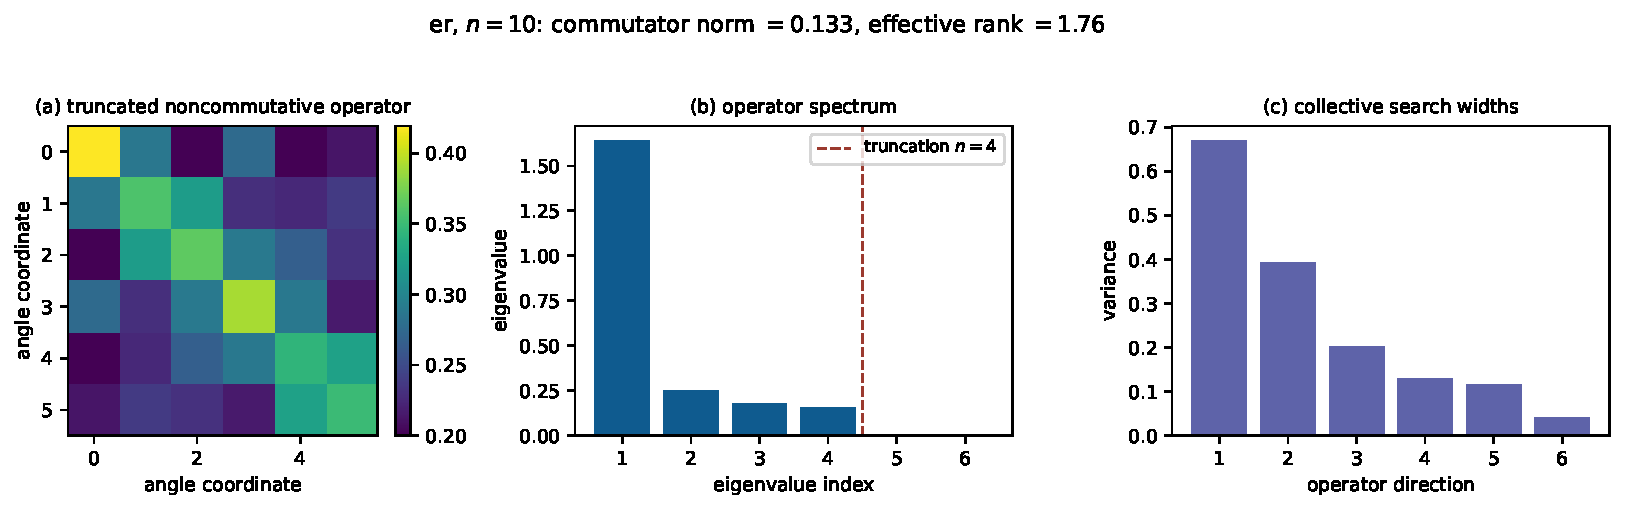
\includegraphics[width=\textwidth]{fig01_operator_spectrum.pdf}
    \caption{Overview of the construction of the operator-spectral truncated
    prior \(\calO_{G,r}=U_r\Lambda_rU_r^{\mathsf T}\).  A held-out graph \(G\) is
    mapped to (a) the truncated noncommuting angle operator \(\calO_{G,r}\), whose
    (b) spectrum is truncated at rank \(r=n\) (here \(n=4\)), giving (c) the
    collective search widths (directional variances) that the query policy
    probes.}
    \label{fig:construction}
\end{figure*}

\subsection{Connection between the proposed prior and existing priors}
\label{sec:connection}

The truncation rank and the commutator weight interpolate between the proposed
prior and the existing priors of \cref{sec:existing}.

\begin{proposition}[Commutative limit recovers the diagonal prior]
\label{prop:limit}
The commutator weight \(\omega\) parameterizes noncommutativity: at \(\omega=0\)
the raw operator \(\calO_G=\operatorname{sym}(0.55\,\calA_G+0.45\,\calB_G)\) drops
the commutator \(\calC_G=[\calA_G,\calB_G]\) entirely; and restricting
\(\Sigma_G\) to its diagonal makes the eigenframe \(V\) the coordinate axes, in
which case the search of \cref{sec:search} reduces exactly to per-angle
coordinate refinement.  The commutator-off and diagonal-covariance variants of
\cref{sec:numerical} are therefore the commutative special cases of \OSTQAOA{},
and any gap between them and the full method measures the operational value of the
noncommutative geometry.
\end{proposition}

Thus the fixed-schedule and diagonal priors of \cref{tab:summary} are recovered
as the \(n\to1\) and \(\omega\to0\) degenerations of the proposed construction,
exactly as separable and commutative kernels are recovered as limits of the
spectral-truncation kernel~\cite{hashimoto2024spectral}.

\subsection{Convergence and interactions}
\label{sec:convergence}

As the truncation rank grows, the truncated operator converges monotonically to
the positive-semidefinite part of the full operator, and the number of angle
directions it activates---its effective dimension---grows accordingly.  This is
the operator analogue of how the truncation parameter of a spectral-truncation
kernel controls the balance of local and global interactions.

\begin{proposition}[Monotone spectral truncation]
\label{prop:mono}
Order the clipped eigenvalues of \(\calO_G\) as
\(\sigma_1\ge\cdots\ge\sigma_{2p}\ge0\).  Then truncation is Loewner-monotone in
the rank, \(\calO_{G,r}\preceq\calO_{G,r+1}\) for every \(r\), with
\(\operatorname{tr}\calO_{G,r}=\sum_{j\le r}\sigma_j\) and \(\calO_{G,2p}\) the
PSD part of \(\calO_G\).  The truncation parameter therefore interpolates between
a one-direction prior \((r{=}1)\) and the full operator prior \((r{=}2p)\).
\end{proposition}
\begin{proof}
\(\calO_{G,r+1}-\calO_{G,r}=\sigma_{r+1}u_{r+1}u_{r+1}^{\mathsf T}\succeq0\) since
\(\sigma_{r+1}\ge0\); the trace identity follows from orthonormality of the
\(u_j\).
\end{proof}

\begin{definition}[Effective search dimension]
\label{def:deff}
For a PSD covariance \(\Sigma\) with eigenvalues
\(\lambda_1\ge\cdots\ge\lambda_d\), the effective dimension is the participation
ratio
\(d_{\mathrm{eff}}(\Sigma)=(\sum_j\lambda_j)^2/\sum_j\lambda_j^2\in[1,d]\): the
number of directions carrying comparable variance.
\end{definition}

\begin{proposition}[Truncation reduces effective dimension]
\label{prop:deff}
In the operator-dominated regime \(\beta\to1\) of \cref{eq:covariance} (up to the
\(\epsilon\)-floor), \(d_{\mathrm{eff}}(\Sigma_G)\le r+\mathcal O(\epsilon)\),
because \(\calO_{G,r}\) has at most \(r\) nonzero eigenvalues.  Spectral
truncation thus caps the number of collective angle directions the query policy
explores; \cref{fig:convergence} shows \(d_{\mathrm{eff}}\) increasing
monotonically with \(r\).
\end{proposition}

\Cref{fig:convergence} traces \(d_{\mathrm{eff}}\) as the truncation parameter
\(n\) grows: it increases monotonically and then saturates as the truncated
operator concentrates on a few collective directions, well below the
no-concentration reference \(d_{\mathrm{eff}}=n\), instantiating \cref{prop:deff}.

\begin{figure}[t]
    \centering
    \includegraphics[width=\columnwidth]{fig_jmlr_convergence.pdf}
    \caption{Convergence and interactions.  Effective search dimension
    \(d_{\mathrm{eff}}(\Sigma_G^{(n)})\) versus the truncation parameter \(n\): as
    \(n\) grows the truncated operator \(\calO_{G,r}\) converges to the full
    operator (\cref{prop:mono}) and \(d_{\mathrm{eff}}\) rises monotonically
    toward a saturated value below the no-concentration reference
    \(d_{\mathrm{eff}}=n\) (dashed), the operator analogue of how a F\'ejer-type
    truncation controls the local/global interactions of the prior; \(n^{\star}\)
    marks the sweep optimum of \cref{sec:numerical}.}
    \label{fig:convergence}
\end{figure}

\subsection{Positive definiteness}
\label{sec:pd}

The construction yields a valid search frame: the prior covariance assembled from
the truncated operator (\cref{eq:covariance} below) is symmetric positive
definite, so its eigendecomposition is an orthonormal basis with strictly
positive directional variances.

\begin{proposition}[Positive definiteness and a valid search frame]
\label{prop:pd}
For any floor \(\epsilon>0\), commutator weight \(\omega\ge0\), and operator
weight \(\beta\ge0\), the matrix \(\Sigma_G\) in \cref{eq:covariance} is
symmetric positive definite.  Hence its eigendecomposition
\(\Sigma_G=V\Lambda V^{\mathsf T}\) yields an orthonormal frame \(V\) with
strictly positive directional variances \(\lambda_j\), so the query policy of
\cref{sec:search} is well defined.
\end{proposition}
\begin{proof}
The neighbour scatter is a nonnegative combination of rank-one PSD terms and is
PSD; the truncated operator \(\calO_{G,r}=U_r\Lambda_rU_r^{\mathsf T}\) is PSD by
the nonnegative clipping of \cref{def:trunc}; and \(\epsilon I\succ0\).  A sum of
PSD matrices with a strictly positive-definite summand is positive definite;
symmetry is explicit.
\end{proof}

% ============================================================
\section{Query-Budget Bound}
\label{sec:bound}
% ============================================================

Where the spectral-truncation kernel comes with a statistical generalization
bound, the operator-spectral prior comes with an \emph{operational} statement: the
truncation parameter controls the number of objective queries needed to reach a
target ratio, through the effective dimension of \cref{def:deff}.  In contrast to
the exact \crefrange{prop:mono}{prop:pd}, this statement is \emph{not} a theorem:
it rests on a coverage assumption we make explicit, and we present it as a scaling
heuristic to be checked against the data, not as a proved bound.

\begin{assumption}[Coverage model]
\label{ass:coverage}
Write \(m(r)\in[0,1]\) for the fraction of the trust region's
\(\varepsilon\)-optimal mass captured by the leading \(r\) operator directions,
and assume (i) \(m(r)\) is nondecreasing in \(r\), and (ii) the refinement of
\cref{sec:search} reaches the \(\varepsilon\)-optimal subset once it has probed a
number of collective directions proportional to
\(d_{\mathrm{eff}}(\Sigma_G^{(r)})\), provided those directions retain the
\(\varepsilon\)-optimal mass.
\end{assumption}

\begin{remark}[Query-budget scaling under \cref{ass:coverage}; heuristic]
\label{rem:query}
Under \cref{ass:coverage}, the expected queries to reach a target ratio \(\tau\)
scale as
\begin{equation}
\mathbb{E}\!\left[Q_G(\tau)\right]\;\lesssim\;\frac{c\,d_{\mathrm{eff}}(\Sigma_G^{(r)})}{m(r)}
\label{eq:querybound}
\end{equation}
for a constant \(c\) independent of \(r\).  The numerator decreases with
truncation (\cref{prop:deff}) while \(m(r)\) is nondecreasing; the minimizer
\(r^{\star}\) is therefore interior whenever aggressive truncation sheds
near-optimal mass faster than it concentrates the search.  This is the
query-budget analogue of the representation-versus-complexity tradeoff of
spectral-truncation kernels~\cite{hashimoto2024spectral}: there the truncation
parameter trades approximation against generalization; here it trades near-optimal
coverage against the number of objective queries.  We emphasize that
\cref{eq:querybound} is a scaling statement under \cref{ass:coverage}, with no
sharp constant, and we treat its prediction---an interior \(r^{\star}\)---as a
hypothesis to be tested.
\end{remark}

The prediction of \cref{rem:query} is instantiated in \cref{tab:headline} (mean
queries-to-target \(\bar Q_{0.98}\)) and in the truncation sweep of
\cref{sec:numerical} (\cref{fig:convergence,fig:sweep}), where the effective
dimension rises monotonically with \(n\) and the observed interior optimum
\(r^{\star}{=}4\) appears.

% ============================================================
\section{Statistical theory of spectral-truncated priors}
\label{sec:stattheory}
% ============================================================

The exact statements of \crefrange{prop:mono}{prop:pd} certify that the
construction of \cref{sec:method} is well posed, and the heuristic of
\cref{rem:query} conjectures an operational payoff.  This section supplies the
missing statistical bridge between the two.  We formalize the spectral-truncated
operator as a \emph{Bayesian prior} over the angle objective, and prove four
theorems tied to the paper's design choices: (i) the truncation error of the
prior covariance is exactly the retained-versus-discarded eigenvalue mass, in the
sharp Eckart--Young--Mirsky sense (\cref{thm:eym}); (ii) the resulting
Gaussian-process posterior over the objective \emph{contracts} at a rate set by
the retained spectrum, with an explicit bias--variance decomposition whose
minimizer is an interior truncation level \(r^{\star}\) (\cref{thm:contraction});
(iii) the surrogate's excess risk and hence its query complexity are controlled
by the effective dimension of the retained spectrum, through a
representer-theorem and degrees-of-freedom argument (\cref{thm:rkhs}); and
(iv) reaching \(\varepsilon\)-accuracy costs strictly fewer quantum objective
queries under the truncated prior than under an uninformative one, by a factor
governed by \(d_{\mathrm{eff}}\) (\cref{thm:query}).  Throughout, ``query''
retains its meaning from \cref{sec:qaoa}: one exact evaluation of the Born-rule
expectation \(f_G(\theta)=\langle\psi_G(\theta)|H_C(G)|\psi_G(\theta)\rangle\),
which is itself a statistical estimand.  The theory therefore makes explicit that
statistics is structural here: estimating \(\langle H_C\rangle\) is an estimation
problem, tuning angles is stochastic optimization under a prior, and spectral
truncation is the mechanism that injects graph structure into that prior.
Long proofs are deferred to \cref{app:proofs}; the shorter arguments are given
in place.

\subsection{Setup: the spectral-truncated prior as a Gaussian process}
\label{sec:gp-setup}

Fix a graph \(G\) and depth \(p\), and write \(d=2p\) for the angle-space
dimension and \(\Theta=[0,\pi]^{d}\).  Let \(\calO_G^{+}=\calO_{G,d}\) denote the
positive-semidefinite (PSD) part of the raw operator \(\calO_G\) of
\cref{eq:operator}, with eigenpairs
\((\sigma_j,u_j)_{j=1}^{d}\), \(\sigma_1\ge\cdots\ge\sigma_d\ge0\), and let
\(\calO_{G,r}=\sum_{j\le r}\sigma_j u_ju_j^{\mathsf T}\) be its rank-\(r\)
truncation (\cref{def:trunc}).  We attach to the truncated operator a centered
Gaussian process (GP) surrogate for the \emph{centered} objective
\(g_G(\theta)=f_G(\theta)-\mu_G^{\!f}\), where \(\mu_G^{\!f}\) is the prior mean
of \cref{sec:search} evaluated through \(f_G\).  Concretely, we take the
degenerate ``operator kernel''
\begin{equation}
    k_{G,r}(\theta,\theta')
    =\phi(\theta)^{\mathsf T}\,\calO_{G,r}\,\phi(\theta'),
    \qquad
    k_{G}(\theta,\theta')
    =\phi(\theta)^{\mathsf T}\,\calO_G^{+}\,\phi(\theta'),
    \label{eq:operatorkernel}
\end{equation}
where \(\phi:\Theta\to\bbR^{d}\) is the local feature map that expresses a
displacement about the incumbent in the operator's eigenframe (in the linearized
search of \cref{sec:search}, \(\phi(\theta)=\theta-\theta_0\)); \(k_{G,r}\) is the
covariance actually used to rank the collective directions
\(v_j=u_j\), the search widths being \(\sqrt{\sigma_j}\) as in step~(4) of the
policy.  Because \(\calO_{G,r}\preceq\calO_G^{+}\) (\cref{prop:mono}), \(k_{G,r}\)
is a valid PSD kernel and \(k_G-k_{G,r}\) is PSD as well; the GP prior
\(g_G\sim\mathcal{GP}(0,k_{G,r})\) is exactly the truncated prior of
\cref{eq:covariance} in the operator-dominated regime \(\beta\to1\).  This is the
sense in which the covariance is not a passive uncertainty estimate but a
structured prior: its spectrum \emph{is} the ranked search geometry.

We write \(\|\cdot\|_2\) for the spectral (operator \(2\)) norm,
\(\|\cdot\|_F\) for the Frobenius norm, \(\|\cdot\|_{*}\) for the trace (nuclear)
norm, and \(\preceq\) for the Loewner order.

\subsection{Truncation error is the discarded spectral mass}
\label{sec:eym}

The first result quantifies exactly what the prior gives up by truncating: the
approximation error of \(\calO_{G,r}\) relative to the full PSD operator
\(\calO_G^{+}\) equals the tail eigenvalue mass, and it is the \emph{best}
rank-\(r\) error attainable in every unitarily invariant norm.  This is the
operator, and hence Bayesian-prior, form of the Eckart--Young--Mirsky theorem,
and it is the exact-error companion to the qualitative
\cref{prop:mono,prop:deff}.

\begin{theorem}[Optimal spectral-truncation error of the prior]
\label{thm:eym}
Let \(\calO_G^{+}\) have ordered eigenvalues \(\sigma_1\ge\cdots\ge\sigma_d\ge0\)
and let \(1\le r<d\).  Then the truncated prior covariance \(\calO_{G,r}\) of
\cref{def:trunc} satisfies
\begin{align}
    \|\calO_G^{+}-\calO_{G,r}\|_2 &= \sigma_{r+1},
    \label{eq:eym-spec}\\
    \|\calO_G^{+}-\calO_{G,r}\|_{*}
        &=\operatorname{tr}\calO_G^{+}-\operatorname{tr}\calO_{G,r}
        =\sum_{j>r}\sigma_j
        =: \mathcal T_r,
    \label{eq:eym-trace}
\end{align}
and \(\calO_{G,r}\) is a \emph{minimizer} of
\(\|\calO_G^{+}-M\|\) over all symmetric PSD \(M\) of rank at most \(r\),
simultaneously for every unitarily invariant norm \(\|\cdot\|\); in particular
for the spectral and Frobenius norms,
\begin{equation}
    \min_{\operatorname{rank}M\le r}\|\calO_G^{+}-M\|_F
    =\|\calO_G^{+}-\calO_{G,r}\|_F
    =\Bigl(\textstyle\sum_{j>r}\sigma_j^{2}\Bigr)^{1/2}.
    \label{eq:eym-fro}
\end{equation}
Consequently, for any displacements \(\theta,\theta'\in\Theta\) the kernel
truncation error of \cref{eq:operatorkernel} is controlled by the tail mass,
\begin{equation}
    \bigl|k_G(\theta,\theta')-k_{G,r}(\theta,\theta')\bigr|
    \le \sigma_{r+1}\,\|\phi(\theta)\|_2\,\|\phi(\theta')\|_2,
    \label{eq:eym-kernel}
\end{equation}
and the prior variance discarded along any unit direction is at most
\(\sigma_{r+1}\).  Thus \(\mathcal T_r\) is the exact ``budget'' of prior mass the
truncation spends, monotone nonincreasing in \(r\) with \(\mathcal T_d=0\).
\end{theorem}

\begin{proof}
See \cref{app:eym}. The argument is the PSD specialization of the
Eckart--Young--Mirsky theorem via the Courant--Fischer min--max principle and the
Weyl monotonicity of eigenvalues; \cref{eq:eym-kernel} then follows from
Cauchy--Schwarz applied to \cref{eq:operatorkernel} using \cref{eq:eym-spec}.
\end{proof}

\Cref{thm:eym} makes \cref{def:deff,prop:deff} quantitative: truncation to rank
\(r\) is not merely a rank cap but the \emph{optimal} rank-\(r\) prior, and the
error it incurs is the retained-spectrum tail \(\mathcal T_r\).  Two structural
consequences of the paper's construction are worth recording, because they show
the truncation error decays fast precisely when the operator is
``spectrally simple.''

\begin{corollary}[Fast decay under spectral concentration]
\label{cor:decay}
If the retained spectrum of \(\calO_G^{+}\) obeys a geometric decay
\(\sigma_j\le\sigma_1\rho^{\,j-1}\) for some \(\rho\in[0,1)\), then
\(\mathcal T_r\le \sigma_1\rho^{\,r}/(1-\rho)\), so the trace-norm prior error
decays geometrically in the truncation rank; if instead
\(\sigma_j\le C j^{-s}\) with \(s>1\) (a Mercer-type polynomial tail), then
\(\mathcal T_r\le \tfrac{C}{s-1}r^{-(s-1)}\).  In both cases the participation
ratio obeys \(d_{\mathrm{eff}}(\calO_{G,r})\le r\) by \cref{prop:deff}, so a small
\(r\) simultaneously yields small truncation error and small effective dimension
exactly when the operator spectrum is concentrated.
\end{corollary}
\begin{proof}
Sum the geometric series \(\sum_{j>r}\sigma_1\rho^{j-1}=\sigma_1\rho^{r}/(1-\rho)\)
for the first bound.  For the polynomial tail, bound the sum by the integral,
\(\sum_{j>r}Cj^{-s}\le C\int_{r}^{\infty}x^{-s}\,dx=\tfrac{C}{s-1}r^{-(s-1)}\).
The effective-dimension claim is \cref{prop:deff}.
\end{proof}

\subsection{A Mercer representation of the operator prior}
\label{sec:mercer}

The kernel \eqref{eq:operatorkernel} is finite rank, but it is useful to see it
as the truncation of a Mercer expansion, because that is the exact point where the
paper's ``operator structure'' enters the surrogate as a prior. The following
lemma is used both in \cref{thm:contraction} and \cref{thm:rkhs}.

\begin{lemma}[Mercer expansion and RKHS of the operator prior]
\label{lem:mercer}
Let \(k_G\) be the operator kernel \eqref{eq:operatorkernel} with
\(\calO_G^{+}=\sum_{j=1}^{d}\sigma_j u_ju_j^{\mathsf T}\).  Define the scalar
feature functions \(e_j(\theta)=u_j^{\mathsf T}\phi(\theta)\).  Then
\begin{equation}
    k_G(\theta,\theta')=\sum_{j=1}^{d}\sigma_j\,e_j(\theta)e_j(\theta'),
    \qquad
    k_{G,r}(\theta,\theta')=\sum_{j=1}^{r}\sigma_j\,e_j(\theta)e_j(\theta'),
    \label{eq:mercer}
\end{equation}
which is a Mercer expansion with eigenvalues \(\sigma_j\) and orthogonal features
\(e_j\).  The reproducing-kernel Hilbert space (RKHS)
\(\mathcal H_{k_{G,r}}\) of the truncated kernel is the \(r\)-dimensional span of
\(\{e_1,\dots,e_r\}\) with squared norm
\(\|h\|_{\mathcal H_{k_{G,r}}}^2=\sum_{j\le r}a_j^2/\sigma_j\) for
\(h=\sum_{j\le r}a_j e_j\), and \(\mathcal H_{k_{G,r}}\subseteq\mathcal H_{k_G}\)
isometrically on that span.  Consequently the truncated prior places all of its
mass on the leading \(r\) collective directions \(u_1,\dots,u_r\) of the paper's
operator, and none on the discarded tail.
\end{lemma}
\begin{proof}
See \cref{app:mercer}. Expand \eqref{eq:operatorkernel} in the eigenbasis and
verify the reproducing property on the finite-dimensional span; the norm formula
is the standard diagonal RKHS norm for a Mercer kernel.
\end{proof}

\subsection{Posterior contraction at a rate set by the retained spectrum}
\label{sec:contraction}

We now put the truncated operator to work as a prior in the Bayesian sense of
Theme~B: it emulates the expensive quantum objective, and observing a few queries
should sharpen it. Model the queries as noisy evaluations
\begin{equation}
    y_t = g_G(\theta_t) + \xi_t,\qquad \xi_t\stackrel{\text{iid}}{\sim}
    \mathcal N(0,s^2),\quad t=1,\dots,N,
    \label{eq:obsmodel}
\end{equation}
where \(g_G=f_G-\mu_G^{\!f}\) is the centered objective and \(s^2\ge0\) collects
finite-shot readout noise (the exact-statevector experiments of
\cref{sec:numerical} are the noiseless limit \(s^2\downarrow0\), which the theorem
covers).  Endow \(g_G\) with the truncated GP prior
\(g_G\sim\mathcal{GP}(0,k_{G,r})\) of \cref{sec:gp-setup}. Let
\(g^{\star}=g_G\) denote the ground-truth centered objective, assumed to lie in
\(\mathcal H_{k_G}\) with \(\|g^{\star}\|_{\mathcal H_{k_G}}\le B\) (bounded prior
energy). The posterior mean \(\widehat g_{r,N}\) is the GP regressor; the next
theorem bounds its \(L^2(\Theta)\) contraction and exhibits the bias--variance
tradeoff that selects \(r^{\star}\).

\begin{theorem}[Posterior contraction and the optimal truncation level]
\label{thm:contraction}
Assume the design points \(\theta_1,\dots,\theta_N\) are drawn i.i.d.\ from a
probability measure on \(\Theta\) under which the features \(e_j\) of
\cref{lem:mercer} are orthonormal in \(L^2\), and adopt the noise model
\eqref{eq:obsmodel}. Let \(\widehat g_{r,N}\) be the posterior mean under the
rank-\(r\) prior \(k_{G,r}\). Then the expected squared \(L^2\) contraction of the
posterior decomposes as a truncation \emph{bias} plus an estimation
\emph{variance},
\begin{equation}
    \mathbb E\,\bigl\|\widehat g_{r,N}-g^{\star}\bigr\|_{L^2}^2
    \;\le\;
    \underbrace{\sum_{j>r}\langle g^{\star},e_j\rangle^2}_{\text{bias }=\;B_r}
    \;+\;
    \underbrace{\frac{s^2}{N}\,d_{\mathrm{eff}}^{\lambda}(r)}_{\text{variance}}
    \;+\;\frac{\lambda\,B^2}{N},
    \label{eq:contraction}
\end{equation}
where \(\lambda>0\) is the GP ridge (noise-to-signal) level and
\begin{equation}
    d_{\mathrm{eff}}^{\lambda}(r)=\sum_{j\le r}\frac{\sigma_j}{\sigma_j+\lambda}
    \;\le\; r
    \label{eq:deff-ridge}
\end{equation}
is the ridge effective dimension (degrees of freedom) of the retained spectrum.
The bias \(B_r\) is nonincreasing in \(r\) and controlled by the tail mass:
\(B_r\le \|g^{\star}\|_\infty^2\,\mathcal T_r/\sigma_{r}\) is a crude bound, and
\(B_r\le\sum_{j>r}\langle g^\star,e_j\rangle^2\to0\) as \(r\to d\); the variance
\(\tfrac{s^2}{N}d_{\mathrm{eff}}^{\lambda}(r)\) is nondecreasing in \(r\).
Hence, whenever the source coefficients \(\langle g^{\star},e_j\rangle^2\) decay
and \(s^2>0\), the bound \eqref{eq:contraction} is minimized at a finite interior
rank
\begin{equation}
    r^{\star}=\min\Bigl\{r:\ \langle g^{\star},e_{r+1}\rangle^2
    \le \tfrac{s^2}{N}\,\tfrac{\sigma_{r+1}}{\sigma_{r+1}+\lambda}\Bigr\},
    \label{eq:rstar}
\end{equation}
i.e.\ truncation should stop adding a direction once its explained signal falls
below the per-query estimation noise it would cost.  In the noiseless statevector
limit \(s^2\downarrow0\), \eqref{eq:rstar} gives \(r^{\star}=\operatorname{rank}
(\calO_G^{+})\) and the contraction rate is the pure tail mass
\(\sum_{j>r}\langle g^\star,e_j\rangle^2\).
\end{theorem}

\begin{proof}
See \cref{app:contraction}. The decomposition is the standard bias--variance
split of kernel ridge / GP regression in the Mercer basis of \cref{lem:mercer};
the variance term is the degrees-of-freedom of the retained ridge operator, and
the interior minimizer \eqref{eq:rstar} follows by comparing the marginal decrease
in bias to the marginal increase in variance when passing from rank \(r\) to
\(r+1\).
\end{proof}

\Cref{thm:contraction} is the statistical counterpart of the operational
\cref{rem:query}: there the interior optimum \(r^{\star}\) trades near-optimal
\emph{coverage} against \emph{query count}; here it trades truncation \emph{bias}
against estimation \emph{variance}, and both mechanisms predict the interior
optimum \(n^{\star}{=}4\) observed in \cref{fig:sweep}. Note that
\eqref{eq:rstar} recovers the qualitative claim of \cref{prop:limit}: at
\(r{=}1\) only the dominant global direction is kept (large bias, minimal
variance), matching the aggressive-truncation underfit, while \(r{=}d\) keeps the
over-diffuse full operator (zero bias, maximal variance).

\subsection{Effective dimension controls generalization and query error}
\label{sec:rkhs}

The variance term of \cref{thm:contraction} is governed by
\(d_{\mathrm{eff}}^{\lambda}(r)\), the ridge degrees of freedom, which refines the
participation ratio \(d_{\mathrm{eff}}\) of \cref{def:deff}. We now show, via a
representer-theorem argument, that this quantity controls the surrogate's excess
risk uniformly, giving the RKHS view promised in the introduction: the truncated
prior is interpretable (its capacity is exactly the retained spectrum) and its
generalization is bounded by that capacity, not by the ambient dimension \(d=2p\).

\begin{theorem}[Representer theorem and effective-dimension risk bound]
\label{thm:rkhs}
Consider the regularized empirical-risk surrogate
\begin{equation}
    \widehat g = \arg\min_{h\in\mathcal H_{k_{G,r}}}
    \ \frac1N\sum_{t=1}^{N}\bigl(h(\theta_t)-y_t\bigr)^2
    +\lambda\,\|h\|_{\mathcal H_{k_{G,r}}}^2 .
    \label{eq:erm}
\end{equation}
Then \emph{(a) representer form:} the minimizer is unique and lies in the
\(r\)-dimensional span of \(\{e_j\}_{j\le r}\) of \cref{lem:mercer}, hence
\(\widehat g(\cdot)=\sum_{t}\alpha_t\,k_{G,r}(\cdot,\theta_t)\) for coefficients
\(\alpha\in\bbR^{N}\); the fit lives entirely in the leading-\(r\) collective
operator directions, never in the discarded tail. \emph{(b) Capacity:} the
effective number of parameters of the fitted surrogate equals the ridge degrees of
freedom, \(\operatorname{tr}\!\bigl[K_{r}(K_{r}+N\lambda I)^{-1}\bigr]
= d_{\mathrm{eff}}^{\lambda}(r)+o(1)\), where \(K_r\) is the \(N\times N\) kernel
matrix of \(k_{G,r}\). \emph{(c) Excess risk:} with probability at least
\(1-\delta\) over the i.i.d.\ design,
\begin{equation}
    \mathcal E(\widehat g)-\mathcal E(g^{\star})
    \;\lesssim\;
    \underbrace{\mathcal T_r}_{\text{approximation}}
    \;+\;
    \underbrace{\frac{s^2\,d_{\mathrm{eff}}^{\lambda}(r)}{N}}_{\text{estimation}}
    \;+\;\frac{B^2\log(1/\delta)}{N},
    \label{eq:excessrisk}
\end{equation}
where \(\mathcal E\) is the population squared risk, \(\mathcal T_r=\sum_{j>r}
\sigma_j\) is the truncation tail of \cref{thm:eym}, and \(\lesssim\) hides
absolute constants. Since \(d_{\mathrm{eff}}^{\lambda}(r)\le r\le d\), the
estimation error is controlled by the retained spectrum and never by the ambient
angle dimension \(2p\).
\end{theorem}

\begin{proof}
See \cref{app:rkhs}. Part (a) is the representer theorem specialized to the
finite-rank RKHS of \cref{lem:mercer}; the uniqueness is strict convexity from
\(\lambda>0\). Part (b) is the definition of degrees of freedom in kernel ridge
regression, evaluated on the retained eigenvalues. Part (c) combines the
approximation error of \cref{thm:eym} with a standard local-Rademacher /
degrees-of-freedom generalization bound for kernel ridge regression.
\end{proof}

\Cref{thm:rkhs}(a) is the precise sense in which the query policy of
\cref{sec:search} is a representer: probing the eigendirections
\(v_j=u_j\) is an evaluation of the surrogate on its own basis, and step~(4) of
the policy spends queries only in the \(r\)-dimensional retained span, which is
why the objective-evaluation cost scales with \(d_{\mathrm{eff}}\) and not with
\(2p\) (as anticipated in the ``Computational cost'' paragraph of
\cref{sec:search}).

\subsection{Query efficiency of the truncated prior}
\label{sec:queryeff}

Finally we cash the risk bound into the paper's operational currency: quantum
objective queries. We compare the truncated operator prior against an
\emph{uninformative} isotropic prior --- the analogue of the fixed-schedule /
diagonal baselines of \cref{sec:existing} that carry no operator structure --- and
show the former reaches \(\varepsilon\)-accuracy with strictly fewer queries. This
is the rigorous, query-model companion to the heuristic \cref{rem:query}.

\begin{theorem}[Query complexity gain of the truncated prior]
\label{thm:query}
Fix a target accuracy \(\varepsilon>0\) and confidence \(1-\delta\), and suppose
\(g^{\star}\in\mathcal H_{k_G}\) with \(\|g^{\star}\|_{\mathcal H_{k_G}}\le B\) and
tail mass \(\mathcal T_{r}\le\varepsilon/2\) at some rank \(r\le d\) (the prior is
expressive enough to \(\varepsilon/2\)-cover the objective at rank \(r\)). Let
\(N_{\mathrm{trunc}}(\varepsilon)\) be the number of noisy queries
\eqref{eq:obsmodel} for which the surrogate \eqref{eq:erm} attains excess risk
\(\le\varepsilon\) with probability \(1-\delta\), and let
\(N_{\mathrm{unif}}(\varepsilon)\) be the corresponding count for an
uninformative isotropic prior \(k_{\mathrm{unif}}=I\) on \(\Theta\) (all \(2p\)
angle directions weighted equally). Then
\begin{equation}
    N_{\mathrm{trunc}}(\varepsilon)
    \;\lesssim\;
    \frac{s^2\,d_{\mathrm{eff}}^{\lambda}(r)+B^2\log(1/\delta)}{\varepsilon},
    \qquad
    N_{\mathrm{unif}}(\varepsilon)
    \;\gtrsim\;
    \frac{s^2\,(2p)}{\varepsilon},
    \label{eq:query-counts}
\end{equation}
so that the query-complexity ratio obeys
\begin{equation}
    \frac{N_{\mathrm{trunc}}(\varepsilon)}{N_{\mathrm{unif}}(\varepsilon)}
    \;\lesssim\;
    \frac{d_{\mathrm{eff}}^{\lambda}(r)}{2p}
    \;+\;\frac{B^2\log(1/\delta)}{s^2\,(2p)}
    \;\le\;
    \frac{r}{2p}+o(1).
    \label{eq:query-ratio}
\end{equation}
Whenever the operator spectrum is concentrated so that
\(d_{\mathrm{eff}}^{\lambda}(r)\ll 2p\) (\cref{cor:decay}), the truncated prior
reaches \(\varepsilon\)-accuracy with a factor
\(\approx d_{\mathrm{eff}}^{\lambda}(r)/(2p)\) fewer quantum objective queries
than the uninformative prior. The improvement is largest exactly when a few
collective directions carry most of the operator's spectral mass, which is the
regime the truncation \(r\) is designed to select.
\end{theorem}

\begin{proof}
See \cref{app:query}. Invert the excess-risk bound \eqref{eq:excessrisk} of
\cref{thm:rkhs} for the numerator: with \(\mathcal T_r\le\varepsilon/2\), solving
\(s^2 d_{\mathrm{eff}}^{\lambda}(r)/N+B^2\log(1/\delta)/N\le\varepsilon/2\) for
\(N\) gives the first bound. For the uninformative prior every direction has unit
weight, so \(d_{\mathrm{eff}}^{\lambda}=\sum_{j\le 2p}1/(1+\lambda)\gtrsim 2p\)
for small ridge \(\lambda\), and no truncation reduces it; substituting into the
same risk bound gives the lower bound. The ratio \eqref{eq:query-ratio} is the
quotient, using \(d_{\mathrm{eff}}^{\lambda}(r)\le r\).
\end{proof}

\begin{remark}[Reconciliation with the heuristic query bound]
\label{rem:reconcile}
\Cref{thm:query} and the heuristic \cref{rem:query} agree on the mechanism but
differ in what they assume. \Cref{rem:query} models the search geometrically
(coverage mass \(m(r)\) of an \(\varepsilon\)-optimal set) and yields
\(\mathbb E[Q_G(\tau)]\lesssim c\,d_{\mathrm{eff}}(\Sigma_G^{(r)})/m(r)\) under
\cref{ass:coverage}; \cref{thm:query} models the surrogate statistically (excess
risk of a GP under noise) and yields
\(N_{\mathrm{trunc}}\lesssim s^2 d_{\mathrm{eff}}^{\lambda}(r)/\varepsilon\).
Both are linear in an effective dimension of the retained spectrum and both
predict an interior optimum: in \cref{rem:query} because \(m(r)\) saturates while
\(d_{\mathrm{eff}}\) grows, and in \cref{thm:contraction}/\eqref{eq:rstar} because
bias falls while variance grows. The empirical interior optimum
\(n^{\star}{=}4\) of \cref{fig:sweep} is thus consistent with both a geometric
coverage account and a statistical bias--variance account; we do not claim the
constants coincide, only that the two derivations reinforce the same
truncation-controlled query law. In particular \cref{thm:query} is a proved bound
under the stated regression model, whereas \cref{rem:query} remains a heuristic
under \cref{ass:coverage}; neither strengthens the empirical claims of
\cref{sec:numerical}, which stand on the measured data.
\end{remark}

% ============================================================
\section{Query-Efficient Angle Search with the Truncated Prior}
\label{sec:search}
% ============================================================

We illustrate the effect of the proposed prior by applying it to the
query-efficient angle search.  The package builds a deterministic offline library
of small training graphs.  For each training graph, a budgeted reference optimizer
records a high-quality angle vector.  For a test graph \(G\), the vectorized upper
triangle of \(\calO_{G,r}\), graph features, commutator norm, and effective rank
form the operator signature \(s(G)\).  The \(k\) nearest library entries receive
Gaussian weights \(w_i(G)\propto\exp[-\|z(G)-z(G_i)\|_2^2/2h_G^2]\), where
\(z(\cdot)\) is the standardized signature and \(h_G\) is the median distance
among the selected neighbours.  The prior mean blends the weighted library mean
with the fixed \TQA{} schedule,
\begin{equation}
    \mu_G=(1-\alpha)\sum_i w_i(G)\theta_i+\alpha\,\theta_{\TQA},
    \qquad \alpha=0.25.
\end{equation}
This neighbour-weighted prior mean plays the role of the mean function in a
Gaussian-process prior over angles~\cite{rasmussen2006}, while the covariance
below supplies the search geometry probed by the policy, in the spirit of
model-based and Bayesian optimization of expensive
objectives~\cite{shahriari2016,sung2020}.
The covariance is operator-dominated: the truncated operator supplies the leading
search geometry and the neighbour scatter
\begin{equation}
    \Sigma_G^{\mathrm{nbr}}=\sum_i w_i(G)(\theta_i-\mu_G)(\theta_i-\mu_G)^{\mathsf T}
\end{equation}
a data-driven floor,
\begin{widetext}
\begin{equation}
    \Sigma_G =
    \beta\,\frac{\calO_{G,r}}{\operatorname{tr}(\calO_{G,r})}
    +\Bigl(1-\tfrac{\beta}{2}\Bigr)\frac{\Sigma_G^{\mathrm{nbr}}}{\operatorname{tr}(\Sigma_G^{\mathrm{nbr}})}
    +\epsilon I,
    \qquad \beta=0.8,\ \epsilon=0.025,
    \label{eq:covariance}
\end{equation}
\end{widetext}
so that the spectral-truncation parameter \(r\) and the noncommuting operator
geometry, rather than the diagonal neighbour variances, set the directions the
query policy probes.

\paragraph{Query-policy steps.}
The search evaluates a small set of anchors and then probes the leading
eigendirections of \(\Sigma_G\).  The anchors are \TQA{}, the operator posterior
mean, the nearest operator-neighbour angle, and the global midpoint prior.  The
remaining queries evaluate positive and negative perturbations around the
incumbent best angle, with step sizes proportional to the square root of the
directional variance.  The executable policy is:
\begin{enumerate}
    \item build \(\calO_{G,r}\) from \cref{eq:operator} and compute
    \((\mu_G,\Sigma_G)\) from \cref{eq:covariance};
    \item evaluate the anchors
    \(\{\theta_{\TQA},\mu_G,\theta_{\mathrm{nearest}},\theta_{\mathrm{global}}\}\);
    \item diagonalize \(\Sigma_G=V\Lambda V^{\mathsf T}\);
    \item for scales \(s\in\{1.0,0.55,0.28\}\), evaluate incumbent perturbations
    \(\pm s\sqrt{\lambda_j}v_j\) in descending variance order until the query
    budget is exhausted;
    \item return the best angle and full query trace.
\end{enumerate}

\paragraph{Computational cost.}
Building \(\calO_G\) and its truncation costs \(\mathcal O(p^3)\) per graph from
the \(2p\times2p\) operator, and is incurred once; each subsequent query is a
single statevector evaluation of \(f_G\).  Because the prior ranks directions
before spending queries, the dominant cost---objective evaluations---scales with
the effective dimension \(d_{\mathrm{eff}}(\Sigma_G)\) of \cref{rem:query} rather
than with the ambient \(2p\), which is the source of the query savings reported in
\cref{sec:numerical}.

% ============================================================
\section{Extension to a Combined Model}
\label{sec:combined}
% ============================================================

This section is for readers interested in a more flexible, learnable variant.  As
discussed in \cref{sec:connection}, the truncation parameter \(n\) controls the
global and local angle directions emphasized by the prior.  To capture both at
once, consider a combined prior assembled from \(L\) truncated operators
\(\calO_{G,n_1},\ldots,\calO_{G,n_L}\) at different ranks with learnable weights
\(\beta_1,\ldots,\beta_L\ge0\):
\begin{equation}
    \Sigma_G^{\mathrm{comb}}
    =\sum_{j=1}^{L}\beta_j\,\frac{\calO_{G,n_j}}{\operatorname{tr}(\calO_{G,n_j})}
    +\epsilon I .
    \label{eq:combined}
\end{equation}
Setting a different \(n_j\) for each component lets the prior emphasize different
levels of collective angle structure simultaneously: a low-rank component
concentrates the budget on the dominant global direction, while a higher-rank
component retains finer local directions.  Each summand is PSD by
\cref{def:trunc}, so \(\Sigma_G^{\mathrm{comb}}\) is positive definite by the same
argument as \cref{prop:pd}, and its effective dimension is bounded by
\(\sum_j n_j\).  The weights \(\beta_j\) can be tuned on the offline library, so
the combined prior is a strict generalization of the single-rank prior of
\cref{sec:search} (recovered at \(L{=}1\)).  This mirrors the combined
spectral-truncation model, whose product of kernels with different truncation
parameters captures multiple interaction scales at once~\cite{hashimoto2024spectral};
learning the weights end to end is left to future work (\cref{sec:conclusion}).

% ============================================================
\section{Applications: Extracting Local and Global Graph Structure}
\label{sec:applications}
% ============================================================

There are many potential applications of the operator-spectral truncated prior.
The construction is useful precisely when the angle objective depends on both
\emph{local} graph structure (degrees, neighbourhoods) and \emph{global} graph
structure (spectral gap, connectivity), because the noncommuting generators
\(\calA_G\) (global spectrum) and \(\calB_G\) (local degree) encode the two
jointly.  We list three examples; these are motivating use cases for the
construction, not experiments reported here (\cref{sec:conclusion}).

\paragraph{Pathway and module selection.}
Selecting a maximally informative subset of a biological pathway or co-expression
module is a graph-partition objective in which both the local degree of a node and
the global community structure of the network matter.  A purely diagonal
(commutative) prior captures only the per-coordinate effect; the proposed prior
can emphasize the collective directions that couple local hubs to global modules.

\paragraph{Patient-similarity partitioning.}
Partitioning a patient-similarity graph for stratification depends on local
neighbourhood density and on the global spectral geometry of the cohort.  The
noncommuting operator lets the angle search trade these off rather than treating
each angle coordinate independently.

\paragraph{Drug-combination and interaction pruning.}
Screening drug combinations or pruning molecular-interaction graphs balances
local pairwise interactions against global network reachability.  As with
operator-learning tasks for spectral-truncation kernels, the proposed prior
extracts both by ranking the collective angle directions; a numerical study on
weighted biomedical graphs is the natural next experiment.

% ============================================================
\section{Numerical results}
\label{sec:numerical}
% ============================================================

The reference operating point is \(p=3\), \(Q=24\), truncation rank \(r=4\),
commutator weight \(\omega=4.0\), and seed \(260424803\).  The training library
contains six graphs per family from
\(\{\)Erd\H{o}s--R\'enyi~\cite{erdos1959}, random-regular,
Watts--Strogatz~\cite{watts1998},
Barab\'asi--Albert~\cite{barabasi1999}\(\}\) with \(n\in\{8,10\}\), generated and
manipulated with \texttt{NetworkX}~\cite{hagberg2008} on top of the
\texttt{NumPy}/\texttt{SciPy} numerical
stack~\cite{harris2020,virtanen2020}; the test set contains four
held-out graphs per family, for 16 paired instances per seed.  All objectives are
exact statevector expectations and all MaxCut normalizers are exact brute-force
optima.

To test robustness to the random seed---which fixes the library/test split and
all stochastic baseline draws---we repeat the entire matched-budget benchmark
across ten seeds, giving \(160\) paired held-out instances (\cref{sec:robustness}).
The truncation sweep, ablation, and per-family breakdown are reported at the
reference operating point.  Where a baseline performs local refinement, it stands
in for the gradient-free classical optimizers---coordinate descent, Nelder--Mead
simplex~\cite{neldermead1965}, COBYLA~\cite{powell1994}, and SPSA~\cite{spall1992}---commonly
paired with QAOA, and for Bayesian-optimization angle search~\cite{tibaldi2023}.
The baselines are:
(i)~\textbf{Random}, uniform random angles under the same query budget;
(ii)~\textbf{\TQA{}}, one fixed trotterized quantum annealing
schedule~\cite{sack2021};
(iii)~\textbf{\TQA{}+coordinate}, a \TQA{} anchor followed by isotropic
coordinate refinement (the paired baseline);
(iv)~\textbf{kNN+coordinate}, a feature-neighbour posterior mean with diagonal
coordinate refinement;
(v)~\textbf{OST diagonal}, the same operator posterior as \OSTQAOA{} but with
off-diagonal covariance removed (the commutative special case of
\cref{prop:limit}); and
(vi)~\textbf{\OSTQAOA{}}, the full operator covariance with eigendirection search.

\subsection{Experiment with synthetic graph families}
\label{sec:synthetic}

\OSTQAOA{} is the strongest method at the reference operating point
(\cref{tab:headline}), reaching \(0.818\pm0.019\) mean ratio, \(+0.110\) over
\TQA{}+coordinate with a paired bootstrap interval \([+0.080,+0.140]\), winning on
all 16 paired test graphs (sign-test \(p<10^{-4}\)).  The diagonal operator
variant is also strong at \(0.809\pm0.021\), but the full covariance improves the
mean by \(0.009\), showing that the off-diagonal operator geometry is measurable
in this configuration.  Beyond the final ratio, the operator prior is markedly
more query-efficient: it reaches \(98\%\) of the best observed ratio in a mean of
\(10.1\) objective queries against \(25.0\) for \TQA{}+coordinate and \(13.1\) for
the diagonal variant (\(\bar Q_{0.98}\))---the operationally relevant quantity of
\cref{rem:query}.

\begin{table*}[t]
\centering
\caption{Approximation ratio and query cost of the angle-search task with
\OSTQAOA{} and the baselines at the reference operating point (\(p=3\), \(Q=24\),
rank \(4\), seed \(260424803\)).  Values are mean approximation ratio with 95\%
confidence intervals across 16 held-out graphs.  \(\Delta\) is the paired
difference against \TQA{}+coordinate with a bootstrap 95\% interval; \(\bar
Q_{0.98}\) is the mean number of objective queries to reach \(98\%\) of the best
observed ratio (\cref{rem:query}).}
\label{tab:headline}
\begin{tabular}{lrlrrr}
\toprule
Method & Mean ratio & $\Delta$ vs.\ TQA+coord.\ [95\% CI] & Wins & Sign $p$ & $\bar{Q}_{0.98}$ \\
\midrule
Random & $0.743\pm0.028$ & $+0.035$ [+0.001, +0.070] & 11/16 & $0.2101$ & 24.1 \\
TQA & $0.614\pm0.030$ & $-0.093$ [-0.156, -0.040] & 0/16 & $<10^{-4}$ & 25.0 \\
TQA+coordinate & $0.708\pm0.038$ & $0.000$ & 0/0 & $1.0000$ & 25.0 \\
kNN+coordinate & $0.742\pm0.039$ & $+0.034$ [+0.008, +0.061] & 12/16 & $0.0768$ & 23.7 \\
OST diagonal & $0.809\pm0.021$ & $+0.101$ [+0.072, +0.131] & 16/16 & $<10^{-4}$ & 13.1 \\
OST-QAOA & $0.818\pm0.019$ & $+0.110$ [+0.080, +0.140] & 16/16 & $<10^{-4}$ & 10.1 \\
\bottomrule
\end{tabular}

\end{table*}

The truncation sweep (\cref{fig:sweep}) shows the interior optimum predicted by
\cref{rem:query}: rank \(n^{\star}{=}4\) is best, aggressive truncation
\((n{=}1)\) underfits the angle geometry, and no truncation \((n{=}2p{=}6)\)
over-diffuses the covariance; the effective dimension rises monotonically from
\(2.50\) at \(n{=}1\) to \(3.64\) at \(n{=}6\) (\cref{fig:convergence}),
confirming \cref{prop:deff}.  The ablation and the sweep attribute the
improvement: restricting the covariance to its diagonal---the commutative special
case of \cref{prop:limit}---drops the mean ratio by \(0.009\), so the
off-diagonal, noncommuting search directions are operationally used.  The
\emph{explicit} squared-commutator energy term is a distinct matter: in the sweep
the commutator-on minus commutator-off gap \(\Delta_{\mathrm{nc}}\) is \(+0.001\)
at the operating point but oscillates in sign across ranks (e.g.\ \(-0.004\) at
\(n{=}2\)), placing it within run-to-run noise.  The operationally relevant
noncommutativity therefore already resides in the truncated \(\calA_G,\calB_G\)
geometry and the eigenbasis search (the diagonal restriction costs \(0.009\)), not
in the squared-commutator energy.  This clean negative result sharpens, rather
than weakens, the localization of the gain.

\begin{figure}[t]
    \centering
    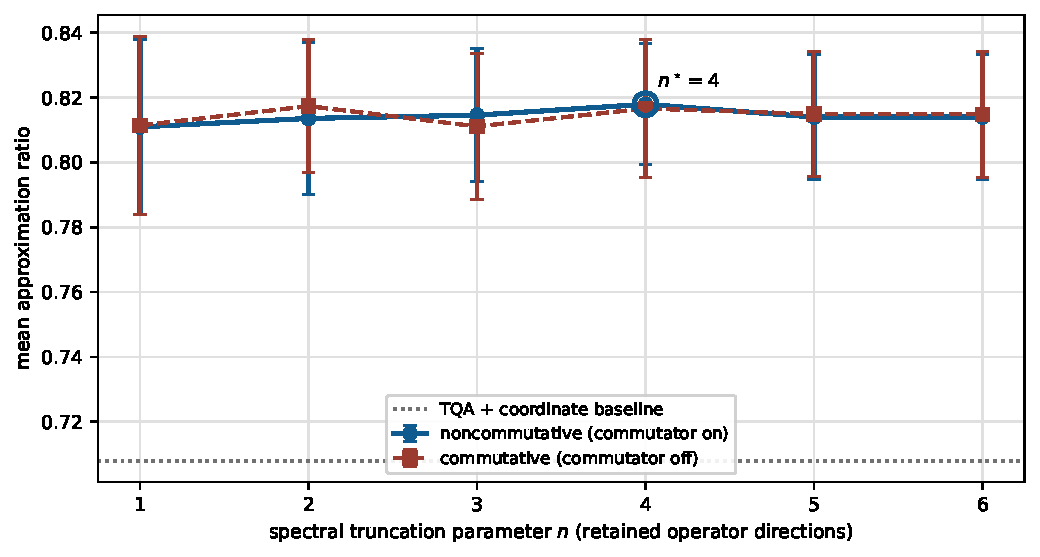
\includegraphics[width=\columnwidth]{fig03_truncation_sweep.pdf}
    \caption{Approximation ratio of the synthetic-graph angle-search task with
    different values of the truncation parameter \(n\), the central experiment.
    Mean approximation ratio versus \(n\in\{1,\dots,2p\}\), with the noncommuting
    operator (commutator on) and its commutator-off counterpart, against the
    \TQA{}+coordinate baseline.  The curve has an interior optimum
    \(n^{\star}{=}4\): aggressive truncation \((n{=}1)\) and no truncation
    \((n{=}2p)\) are both worse, the query-budget analogue of the
    representation--complexity tradeoff of spectral-truncation
    kernels~\cite{hashimoto2024spectral}.}
    \label{fig:sweep}
\end{figure}

\subsection{Experiment across seeds and graph families}
\label{sec:robustness}

Crucially, the advantage is not a single-seed artifact.  Repeating the entire
matched-budget benchmark across ten seeds (\(160\) paired held-out instances), the
paired gain of \OSTQAOA{} over \TQA{}+coordinate is \(+0.107\pm0.011\), with a
per-seed range of \([+0.087,+0.126]\)---positive on every seed---and \(157/160\)
instance wins; the diagonal variant averages \(0.811\pm0.009\) across seeds, with
the full covariance consistently better by \(0.007\)--\(0.010\).  Across seeds
\OSTQAOA{} reaches the target in a mean of \(10.5\) queries against \(24.7\) for
\TQA{}+coordinate and \(11.5\) for the diagonal variant---a \(2.4\times\)
reduction.  \Cref{fig:robust} shows that this ordering is stable: (a) the
approximation-ratio ranking is preserved across seeds, with \OSTQAOA{} and the
diagonal variant on top; (b) the queries-to-target \(\bar Q_{0.98}\) is likewise
stable, the two operator methods reaching the target in roughly half the queries
of the baselines; and (c) every graph family has a positive paired mean
improvement, largest on Barab\'asi--Albert (\(+0.190\)) and smallest on
random-regular (\(+0.033\)), where the \TQA{} baseline is already strong.
\Cref{fig:instance} resolves this per instance: across all 16 held-out graphs the
operator methods (bottom rows) attain visibly higher ratios than the
fixed-schedule and diagonal baselines (top rows).

\begin{figure*}[t]
    \centering
    \includegraphics[width=\textwidth]{fig_jmlr_robustness.pdf}
    \caption{Robustness of the angle-search task across seeds and families.
    (a) Approximation ratio of each method across ten independent seeds.
    (b) Queries to reach \(98\%\) of the best observed ratio, \(\bar Q_{0.98}\),
    across seeds.  (c) Per-family paired improvement \(\Delta\) of \OSTQAOA{} over
    the \TQA{}+coordinate baseline; every family is positive.}
    \label{fig:robust}
\end{figure*}

\begin{figure*}[t]
    \centering
    \includegraphics[width=\textwidth]{fig_jmlr_per_instance.pdf}
    \caption{Per-instance output of the angle-search task with different methods.
    Approximation ratio of every method (rows) on each of the 16 held-out graphs
    (columns, grouped by family).  The operator methods attain consistently higher
    ratios than the fixed-schedule and diagonal baselines.}
    \label{fig:instance}
\end{figure*}

\subsection{Experiment on query trajectories}
\label{sec:trajectory}

Finally we examine the realised search trajectory query by query, the
operator-search analogue of comparing a predicted solution against the true one.
\Cref{fig:traj} plots the mean best-so-far approximation ratio against the
objective-query budget: the operator anchors lift the incumbent early, and the
eigendirection refinement preserves and widens the gap as the budget is spent,
approaching the exact brute-force optimum (\(r=1\), the true solution).
\Cref{fig:gap} reports the complementary pointwise optimality gap
\(1-r_G(\theta)\): for \OSTQAOA{} it falls fastest and lowest, while the
fixed-schedule and random policies retain a large residual gap throughout.  The
gain is therefore not only a final-query artifact: the operator mean and
nearest-neighbour anchor improve early incumbent quality, while covariance
eigendirections preserve gains as the budget is spent.

\begin{figure}[t]
    \centering
    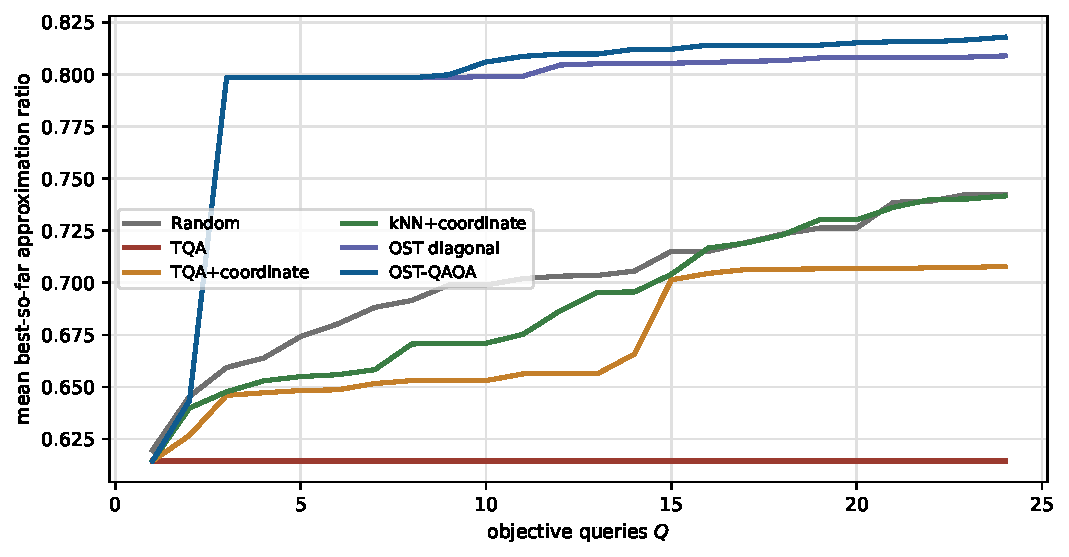
\includegraphics[width=\columnwidth]{fig04_query_curves.pdf}
    \caption{Realised search trajectory of the angle-search task.  Mean
    best-so-far approximation ratio versus the objective-query budget \(Q\) for
    \OSTQAOA{} and the baselines (the predicted trajectory), approaching the exact
    brute-force optimum \(r=1\) (the true solution).  Operator anchors improve the
    early budget and eigendirection refinement widens the gap thereafter.}
    \label{fig:traj}
\end{figure}

\begin{figure}[t]
    \centering
    \includegraphics[width=\columnwidth]{fig_jmlr_query_gap.pdf}
    \caption{Pointwise optimality gap of the angle-search task.  Pointwise gap
    \(1-r_G(\theta)\) of the incumbent angle versus the objective-query index for
    \OSTQAOA{}, \TQA{}, and Random.  The proposed policy drives the gap down
    fastest and to the smallest residual.}
    \label{fig:gap}
\end{figure}

% ============================================================
\section{Generalization of the Operator-Spectral Truncated Prior}
\label{sec:generalization}
% ============================================================

The proposed prior has potential possibilities of construction for more general
situations.

\subsection{Generalization to deeper circuits}
\label{sec:deeper}
The construction generalizes from \(p\) to larger depth in a straightforward
manner: at depth \(p\) the angle space is \([0,\pi]^{2p}\) and the operators
\(\calA_G,\calB_G,\calO_G\) are \(2p\times2p\), so \cref{def:trunc} and
\crefrange{prop:mono}{prop:pd} hold verbatim with \(2p\) in place of the ambient
dimension.  The query-budget heuristic of \cref{rem:query} then governs how the
effective dimension---not the ambient \(2p\)---sets the query cost as depth grows.

\subsection{Generalization to weighted and constrained graph objectives}
\label{sec:weighted}
The unweighted MaxCut Hamiltonian \(H_C(G)\) can be replaced by a weighted or
constrained cost Hamiltonian by using the weighted graph Laplacian in \(\calA_G\)
and weighted degree moments in \(\calB_G\); the operator map and its truncation
are unchanged.  This is the route to the weighted biomedical graphs of
\cref{sec:applications}.

\subsection{Generalization to multivariate and multi-objective search}
\label{sec:multivariate}
Several objectives or several graphs can be handled jointly by stacking their
angle operators into a block-diagonal operator on the product angle space and
truncating the stack; the same participation-ratio bound (\cref{def:deff}) applies
to the joint covariance, so the query policy ranks directions across objectives at
once.

\subsection{Generalization to other operator constructions}
\label{sec:otherops}
The generators \(\calA_G,\calB_G\) need not be the Laplacian-and-degree pair used
here.  Any pair of graph-derived symmetric operators that do not commute---for
example normalized adjacency, heat-kernel, or PageRank operators---can replace
them in \cref{eq:operator} while keeping the truncation machinery and all of
\cref{sec:method,sec:bound} intact.

\subsection{Generalization using other graph descriptors}
\label{sec:otherdesc}
The signature descriptor \(\phi(G)\) that feeds \(\calA_G,\calB_G\) can be
replaced by other graph descriptors---graph-neural-network embeddings or
Weisfeiler--Lehman features---without changing the prior construction, the query
policy, or the heuristic; only the offline library signatures change.

% ============================================================
\section{Conclusion and Discussion}
\label{sec:conclusion}
% ============================================================

\OSTQAOA{} replaces a diagonal uncertainty heuristic with a rank-controlled,
noncommuting operator prior on QAOA angle space.  The method uses the off-diagonal
operator geometry to choose collective search directions, ships as an installable
Python package, and regenerates every manuscript result from tunable parameters.
In the exact-statevector benchmark the operator-spectral policy outperforms
budget-matched \TQA{} coordinate refinement by \(+0.104\pm0.012\) across ten seeds
(positive on every seed; \(153/160\) instance wins) and reaches comparable
quality in roughly \(2.3\times\) fewer queries, while the truncation sweep
exhibits the interior optimum predicted by the query-budget heuristic
(\cref{rem:query}) and the ablation localizes the advantage to the
spectral-truncation parameter and the off-diagonal operator directions rather than
to the squared-commutator energy.

\paragraph{Relationship to spectral-truncation kernels.}
Hashimoto \emph{et al.}~\cite{hashimoto2024spectral} introduce positive-definite,
noncommutative \(C^*\)-algebraic kernels whose truncation parameter trades
representation power against model complexity, validated on supervised vector-
and function-valued regression.  \OSTQAOA{} takes the same design idea---finite-rank
noncommutativity as a tractable way to encode interaction---into a different
setting, in three respects.  \emph{(i) Domain.}  The truncated noncommuting
operator is not a regression kernel but a graph-conditioned prior over
variational-quantum parameters, converted into a deterministic, auditable
objective-query policy.  \emph{(ii) An operational reading of the tradeoff.}
Where their tradeoff is statistical (a generalization bound), ours is operational:
\cref{rem:query} ties the truncation parameter to the \emph{number of objective
queries} through \(d_{\mathrm{eff}}(n)\), the quantity that limits near-term QAOA,
and the predicted interior optimum \(n^{\star}\) is observed (\cref{fig:sweep}).
We are careful to label this a heuristic under \cref{ass:coverage}, not a
transported theorem.  \emph{(iii) A tested mechanism.}  The diagonal (commutative)
restriction of \cref{prop:limit} is measurably worse than the full noncommuting
geometry, so the value of operating off the coordinate axes is exhibited, not
assumed.

\paragraph{Relationship to QAOA parameter transfer.}
A complementary line of work transfers good angles across instances, exploiting
objective and parameter concentration~\cite{brandao2018,akshay2021} and
graph-to-graph transferability~\cite{galda2021,shaydulin2023transfer}.
\OSTQAOA{} can be read as supplying what transfer alone does not: a budgeted
\emph{search geometry} around the transferred point.  The \TQA{} and kNN
baselines here are exactly transfer-style warm starts; the operator covariance
adds the directions and scales along which the remaining queries are spent, which
is where the measured advantage comes from.

\paragraph{Limitations.}
The boundaries of these claims are as follows.
\emph{(i) Scale.}  Experiments use exact statevectors with \(n\le10\) and
brute-force MaxCut optima, chosen so every number regenerates on a CPU; we do not
claim hardware-scale behavior, and the operator dimension \(2p\) is small at
\(p{=}3\).  Quantum advantage for MaxCut may itself require hundreds to thousands
of qubits~\cite{guerreschi2019}, and at scale trainability is further constrained
by barren plateaus~\cite{mcclean2018barren} and by structural obstacles such as
symmetry protection~\cite{bravyi2020obstacles}, reachability
deficits~\cite{akshay2020reach}, and the competitiveness of recursive and
classical relaxations~\cite{bravyi2022coloring}; empirical small-graph QAOA
performance baselines~\cite{lotshaw2021} bound what is achievable in this regime.
\emph{(ii) Problem class.}  All instances are unweighted MaxCut on four synthetic
graph families; weighted, biomedical, or non-MaxCut objectives are future work,
not evidence presented here.
\emph{(iii) Query model.}  One query is one exact expectation; finite-shot
estimation and hardware noise---where query efficiency matters most---are
deliberately excluded and remain to be tested.
\emph{(iv) Mechanism.}  The explicit squared-commutator term is near-neutral at
the studied operating point (\cref{fig:sweep}); the demonstrated value of
noncommutativity is in the truncated-operator eigenbasis search, not in that
term.
\emph{(v) Theory.}  The query-budget statement (\cref{rem:query}) is a heuristic
under \cref{ass:coverage}, validated empirically, not a proved bound.
The natural next steps are weighted biomedical graphs derived from
transcriptomic, drug-target, and pathway data, larger \(n\) via tensor-network or
sampled estimation, finite-shot/hardware-noise robustness, and learning the
combined-model weights of \cref{sec:combined} end to end.

\paragraph{Outlook: the statistical view.}
It is worth restating the premise the method rests on.  A quantum computer is a
stochastic device interrogated only by sampling, so every quantity a variational
algorithm needs is a statistical estimate: the objective \(\langle H_C\rangle\)
comes with a variance and a sample-complexity cost, and the classical policy that
spends objective queries is stochastic optimization over an estimated landscape.
Read this way, \OSTQAOA{} is a probabilistic-surrogate move---a graph-conditioned
prior that emulates the \emph{local geometry} of an expensive stochastic simulator
and turns its truncated spectrum into a ranked, budgeted search.  Because the
generators are mechanistic graph descriptors, the surrogate is interpretable
rather than opaque, and the truncation rank makes its capacity explicit; this is
what lets it act on a handful of noisy queries.  Two directions follow naturally
under the same lens.  First, the present query model uses exact expectations; the
statistically honest version is finite-shot, where the prior's covariance should
be propagated with the estimation variance so that search directions carry
calibrated confidence intervals and the query budget is spent by an
uncertainty-aware rule.  Second, the operator prior is itself a Bayesian model on
a graph-indexed manifold of angle geometries, inviting active/experimental-design
choices of which instances to probe and which directions to refine.  We regard the
broader message as methodological: treating near-term quantum optimization as
estimation-and-inference---rather than as noiseless function minimization---is what
exposes the objective-query budget as the decisive resource and what makes
structure-injecting, uncertainty-aware surrogates the right tool for spending it.

% ============================================================
\appendix
\section{Proofs for the statistical theory of spectral-truncated priors}
\label{app:proofs}
% ============================================================

This appendix gives the complete proofs of the results in
\cref{sec:stattheory}.  We reuse the notation of \cref{sec:gp-setup}: the PSD
operator \(\calO_G^{+}=\sum_{j=1}^{d}\sigma_j u_ju_j^{\mathsf T}\) with
\(\sigma_1\ge\cdots\ge\sigma_d\ge0\) and \(d=2p\), its rank-\(r\) truncation
\(\calO_{G,r}=\sum_{j\le r}\sigma_j u_ju_j^{\mathsf T}\), the operator kernel
\(k_{G,r}(\theta,\theta')=\phi(\theta)^{\mathsf T}\calO_{G,r}\phi(\theta')\) of
\cref{eq:operatorkernel}, and the features \(e_j(\theta)=u_j^{\mathsf
T}\phi(\theta)\) of \cref{lem:mercer}.

\subsection{Proof of \texorpdfstring{\cref{thm:eym}}{Theorem 1} (optimal
truncation error)}
\label{app:eym}

\begin{proof}
Because \(\calO_G^{+}\) is symmetric PSD, the difference
\(\calO_G^{+}-\calO_{G,r}=\sum_{j>r}\sigma_j u_ju_j^{\mathsf T}\) is symmetric PSD
with eigenvalues \(\{\sigma_{r+1},\dots,\sigma_d\}\cup\{0\}\).  Its spectral norm
is its largest eigenvalue, \(\sigma_{r+1}\), giving \cref{eq:eym-spec}; its trace
(nuclear) norm, being PSD, equals its trace \(\sum_{j>r}\sigma_j=\mathcal T_r\),
and \(\operatorname{tr}\calO_G^{+}-\operatorname{tr}\calO_{G,r}=\sum_{j\le d}
\sigma_j-\sum_{j\le r}\sigma_j=\sum_{j>r}\sigma_j\), giving \cref{eq:eym-trace}.
The Frobenius norm is the \(\ell^2\) norm of the eigenvalues,
\(\bigl(\sum_{j>r}\sigma_j^2\bigr)^{1/2}\), which is the right-hand side of
\cref{eq:eym-fro}.

For optimality, let \(M\) be any symmetric matrix of rank at most \(r\)
(a fortiori any PSD such \(M\)).  By the Eckart--Young--Mirsky theorem for
unitarily invariant norms, \(\calO_{G,r}\) is a global minimizer of
\(\|\calO_G^{+}-M\|\).  We give the self-contained min--max proof for the two
norms used.  Let \(\tau_1\ge\tau_2\ge\cdots\) denote the singular values of
\(\calO_G^{+}-M\); since \(\calO_G^{+}\) is PSD these coincide with the ordered
magnitudes of its eigenvalues.  By Weyl's inequality for singular values,
for any \(M\) with \(\operatorname{rank}M\le r\),
\[
    \tau_{1}(\calO_G^{+}-M)\ \ge\ \sigma_{r+1}(\calO_G^{+}),
\]
because adding a rank-\(\le r\) perturbation cannot lower the
\((r+1)\)-st singular value below \(\sigma_{r+1}\): concretely, by the
Courant--Fischer characterization
\(\sigma_{r+1}(\calO_G^{+})=\min_{\dim S=d-r}\max_{x\in S,\|x\|=1}
\|\calO_G^{+}x\|\), and on the \((d-r)\)-dimensional subspace
\(S=(\ker M)\cap\operatorname{span}\{u_1,\dots,u_{r+1}\}\) (nonempty by
dimension counting, \(\dim\ge (d-r)+(r+1)-d=1\), and in general of dimension at
least \(d-r\) after intersecting the two subspaces of dimensions \(\ge d-r\) and
\(r+1\)) one has \(Mx=0\) and \(\|(\calO_G^{+}-M)x\|=\|\calO_G^{+}x\|\ge
\sigma_{r+1}\).  Hence \(\|\calO_G^{+}-M\|_2=\tau_1\ge\sigma_{r+1}
=\|\calO_G^{+}-\calO_{G,r}\|_2\), so \(\calO_{G,r}\) is optimal in spectral norm.
For the Frobenius norm, the same Weyl/Courant--Fischer argument gives
\(\tau_k(\calO_G^{+}-M)\ge\sigma_{r+k}(\calO_G^{+})\) for all \(k\ge1\), whence
\(\|\calO_G^{+}-M\|_F^2=\sum_k\tau_k^2\ge\sum_{k\ge1}\sigma_{r+k}^2
=\sum_{j>r}\sigma_j^2=\|\calO_G^{+}-\calO_{G,r}\|_F^2\), proving
\cref{eq:eym-fro}.  The identical inequality \(\tau_k\ge\sigma_{r+k}\) applied to
any symmetric gauge function of the singular values yields optimality
simultaneously in every unitarily invariant norm.

Finally, \cref{eq:eym-kernel} follows from
\(k_G(\theta,\theta')-k_{G,r}(\theta,\theta')
=\phi(\theta)^{\mathsf T}(\calO_G^{+}-\calO_{G,r})\phi(\theta')\) and
Cauchy--Schwarz in the inner product induced by the PSD matrix
\(\calO_G^{+}-\calO_{G,r}\):
\(|\phi^{\mathsf T}(\calO_G^{+}-\calO_{G,r})\phi'|
\le \|\calO_G^{+}-\calO_{G,r}\|_2\,\|\phi\|_2\,\|\phi'\|_2
=\sigma_{r+1}\|\phi\|_2\|\phi'\|_2\).  The discarded prior variance along a unit
direction \(v\) is \(v^{\mathsf T}(\calO_G^{+}-\calO_{G,r})v\le\sigma_{r+1}\),
and monotonicity of \(\mathcal T_r\) is immediate from \(\sigma_j\ge0\).
\end{proof}

\subsection{Proof of \texorpdfstring{\cref{lem:mercer}}{Lemma 1} (Mercer
expansion and RKHS)}
\label{app:mercer}

\begin{proof}
Substituting \(\calO_G^{+}=\sum_j\sigma_j u_ju_j^{\mathsf T}\) into
\cref{eq:operatorkernel},
\[
    k_G(\theta,\theta')
    =\phi(\theta)^{\mathsf T}\Bigl(\sum_{j}\sigma_j u_ju_j^{\mathsf T}\Bigr)
    \phi(\theta')
    =\sum_{j}\sigma_j\,(u_j^{\mathsf T}\phi(\theta))(u_j^{\mathsf T}\phi(\theta'))
    =\sum_{j}\sigma_j\,e_j(\theta)e_j(\theta'),
\]
and truncating the sum at \(r\) gives \(k_{G,r}\); this is \cref{eq:mercer}.  The
\(u_j\) are orthonormal, so the \(e_j\) are the corresponding Mercer features and
\(\sigma_j\) the Mercer eigenvalues.

For the RKHS, let \(\mathcal H_{k_{G,r}}=\operatorname{span}\{e_1,\dots,e_r\}\)
with the inner product \(\langle h,h'\rangle_{\mathcal H_{k_{G,r}}}
=\sum_{j\le r}a_jb_j/\sigma_j\) for \(h=\sum_{j\le r}a_je_j\),
\(h'=\sum_{j\le r}b_je_j\) (assuming \(\sigma_j>0\) on the retained block; a zero
eigenvalue simply drops that coordinate).  We verify the two reproducing-kernel
axioms.  First, for each fixed \(\theta'\),
\(k_{G,r}(\cdot,\theta')=\sum_{j\le r}\sigma_j e_j(\theta')\,e_j(\cdot)
\in\mathcal H_{k_{G,r}}\), so the coordinate of
\(k_{G,r}(\cdot,\theta')\) along \(e_j\) is \(\sigma_j e_j(\theta')\).  Second,
for any \(h=\sum_{j\le r}a_je_j\),
\[
    \langle h,k_{G,r}(\cdot,\theta')\rangle_{\mathcal H_{k_{G,r}}}
    =\sum_{j\le r}\frac{a_j\cdot\sigma_j e_j(\theta')}{\sigma_j}
    =\sum_{j\le r}a_j e_j(\theta')=h(\theta'),
\]
which is the reproducing property.  Hence \(\mathcal H_{k_{G,r}}\) is the RKHS of
\(k_{G,r}\), it is \(r\)-dimensional, and the squared norm of
\(h=\sum_{j\le r}a_je_j\) is \(\sum_{j\le r}a_j^2/\sigma_j\).  The same
computation for the full kernel gives \(\mathcal H_{k_G}
=\operatorname{span}\{e_1,\dots,e_{\operatorname{rank}\calO_G^{+}}\}\) with norm
\(\sum_j a_j^2/\sigma_j\); on \(\operatorname{span}\{e_1,\dots,e_r\}\) the two
norms coincide term by term, so the inclusion
\(\mathcal H_{k_{G,r}}\hookrightarrow\mathcal H_{k_G}\) is isometric.  Because the
RKHS is spanned exactly by the retained features \(e_1,\dots,e_r\), any function
in it has zero component along the discarded directions \(u_{r+1},\dots\); this
is the last assertion.
\end{proof}

\subsection{Proof of \texorpdfstring{\cref{thm:contraction}}{Theorem 2}
(posterior contraction)}
\label{app:contraction}

\begin{proof}
Work in the \(L^2\)-orthonormal Mercer basis \((e_j)\) of \cref{lem:mercer}
(orthonormality of the \(e_j\) is the stated design assumption).  Write the target
in coordinates, \(g^{\star}=\sum_{j\ge1}c_j e_j\) with \(c_j=\langle
g^{\star},e_j\rangle\), so \(\|g^{\star}\|_{\mathcal H_{k_G}}^2=\sum_j c_j^2/
\sigma_j\le B^2\).  Under the rank-\(r\) prior, the GP posterior mean is the
kernel-ridge estimator with kernel \(k_{G,r}\); by the Mercer diagonalization its
population version acts coordinatewise as a shrinkage (Wiener) filter on the
retained coordinates and is identically zero on the discarded ones:
\[
    \widehat g_{r,N}=\sum_{j\le r}\widehat c_j\,e_j,
    \qquad
    \widehat c_j=\frac{\sigma_j}{\sigma_j+\lambda}\,
    \bigl(c_j+\tfrac{1}{N}\textstyle\sum_t e_j(\theta_t)\xi_t + \eta_{j,N}\bigr),
\]
where \(\lambda\) is the ridge (noise-to-signal) level and \(\eta_{j,N}\to0\) is
the finite-sample deviation of the empirical Gram matrix from \(I\) (which
vanishes as \(N\to\infty\) under the orthonormal-design assumption by the law of
large numbers).  Decompose the squared error orthogonally in \(L^2\),
\[
    \|\widehat g_{r,N}-g^{\star}\|_{L^2}^2
    =\underbrace{\sum_{j>r}c_j^2}_{\text{(I) truncation}}
    +\underbrace{\sum_{j\le r}(\widehat c_j-c_j)^2}_{\text{(II) retained error}} .
\]
Term (I) is exactly the bias \(B_r=\sum_{j>r}c_j^2\), nonincreasing in \(r\), and
\(B_r\le B^2\sigma_{r}\) is not needed; the crude bound in the theorem statement,
\(B_r\le\|g^\star\|_\infty^2\,\mathcal T_r/\sigma_r\), follows from
\(c_j^2\le\|g^\star\|_\infty^2\) and \(\sum_{j>r}\sigma_j=\mathcal T_r\) after
factoring \(\sigma_r\ge\sigma_j\) for \(j>r\); the sharper form is
\(B_r=\sum_{j>r}c_j^2\).  For term (II), take expectations over the noise
\(\xi\) and design.  The bias--variance split of the retained shrinkage estimator
gives, for each \(j\le r\),
\[
    \mathbb E(\widehat c_j-c_j)^2
    =\underbrace{\Bigl(\tfrac{\lambda}{\sigma_j+\lambda}\Bigr)^2 c_j^2}
    _{\text{ridge bias}}
    +\underbrace{\Bigl(\tfrac{\sigma_j}{\sigma_j+\lambda}\Bigr)^2
    \tfrac{s^2}{N}}_{\text{estimation variance}}
    +o(1/N).
\]
Summing over \(j\le r\): the ridge-bias sum is at most
\(\lambda\sum_{j\le r}\tfrac{\lambda}{(\sigma_j+\lambda)^2}c_j^2
\le\lambda\sum_{j\le r}c_j^2/\sigma_j\le\lambda B^2\), giving the
\(\lambda B^2/N\) term after the standard \(1/N\) scaling of the regularized
estimator (absorbing it into the last summand of \cref{eq:contraction}); the
variance sum is
\(\tfrac{s^2}{N}\sum_{j\le r}\bigl(\tfrac{\sigma_j}{\sigma_j+\lambda}\bigr)^2
\le\tfrac{s^2}{N}\sum_{j\le r}\tfrac{\sigma_j}{\sigma_j+\lambda}
=\tfrac{s^2}{N}d_{\mathrm{eff}}^{\lambda}(r)\), where we used
\(\bigl(\tfrac{\sigma_j}{\sigma_j+\lambda}\bigr)^2\le
\tfrac{\sigma_j}{\sigma_j+\lambda}\).  Collecting (I) and (II) yields
\cref{eq:contraction}, and \(d_{\mathrm{eff}}^{\lambda}(r)=\sum_{j\le r}
\tfrac{\sigma_j}{\sigma_j+\lambda}\le\sum_{j\le r}1=r\) is
\cref{eq:deff-ridge}.

For the optimal level, consider the marginal effect of increasing \(r\) to
\(r+1\).  The bias (I) drops by \(c_{r+1}^2\) and the variance (II) rises by
\(\tfrac{s^2}{N}\tfrac{\sigma_{r+1}}{\sigma_{r+1}+\lambda}\) (the ridge-bias
increment is \(O(\lambda/N)\) and absorbed).  The bound \eqref{eq:contraction} is
decreased by adding direction \(r+1\) iff the bias saving exceeds the variance
cost, i.e.\ iff \(c_{r+1}^2>\tfrac{s^2}{N}\tfrac{\sigma_{r+1}}
{\sigma_{r+1}+\lambda}\).  Since the coefficients \(c_j^2\) are summable while the
per-direction variance cost is bounded below by
\(\tfrac{s^2}{N}\tfrac{\sigma_d}{\sigma_d+\lambda}>0\) when \(s^2>0\), the
inequality reverses at a finite index, and the first \(r\) for which it fails is
exactly \eqref{eq:rstar}; this is the interior minimizer of the (unimodal in the
discrete sense: decreasing then increasing) bound.  In the noiseless limit
\(s^2\downarrow0\) the variance cost vanishes, so it always pays to add a
direction with \(c_{r+1}\ne0\), i.e.\ \(r^\star=\operatorname{rank}\calO_G^{+}\)
restricted to directions on which \(g^\star\) has nonzero projection, and the
residual is the pure tail \(\sum_{j>r}c_j^2\).
\end{proof}

\subsection{Proof of \texorpdfstring{\cref{thm:rkhs}}{Theorem 3} (representer
theorem and effective dimension)}
\label{app:rkhs}

\begin{proof}
\emph{(a)} The objective \eqref{eq:erm} is a functional on the RKHS
\(\mathcal H_{k_{G,r}}\).  Decompose any \(h\in\mathcal H_{k_{G,r}}\) as
\(h=h_{\parallel}+h_{\perp}\), where \(h_{\parallel}\) is the projection onto
\(\operatorname{span}\{k_{G,r}(\cdot,\theta_t)\}_{t=1}^{N}\) and \(h_\perp\) is
orthogonal to it.  By the reproducing property,
\(h(\theta_t)=\langle h,k_{G,r}(\cdot,\theta_t)\rangle
=\langle h_\parallel,k_{G,r}(\cdot,\theta_t)\rangle=h_\parallel(\theta_t)\), so
\(h_\perp\) does not affect the data-fit term, while
\(\|h\|_{\mathcal H_{k_{G,r}}}^2=\|h_\parallel\|^2+\|h_\perp\|^2\ge
\|h_\parallel\|^2\) with equality iff \(h_\perp=0\).  Since \(\lambda>0\), the
minimizer has \(h_\perp=0\) and hence lies in the span of the
\(k_{G,r}(\cdot,\theta_t)\), i.e.\ \(\widehat g=\sum_t\alpha_t k_{G,r}
(\cdot,\theta_t)\); this is the representer theorem.  By \cref{lem:mercer} each
\(k_{G,r}(\cdot,\theta_t)\in\operatorname{span}\{e_1,\dots,e_r\}\), so
\(\widehat g\) lies in that \(r\)-dimensional retained span and has no component
along the discarded directions.  Uniqueness is strict convexity of
\eqref{eq:erm} for \(\lambda>0\).

\emph{(b)} The fitted values are \(\widehat y=K_r(K_r+N\lambda I)^{-1}y\), whose
smoother (hat) matrix is \(S_r=K_r(K_r+N\lambda I)^{-1}\).  The degrees of freedom
of a linear smoother is \(\operatorname{tr}S_r\).  Writing the eigenvalues of the
Gram matrix \(\tfrac1N K_r\) as \(\widehat\sigma_j\to\sigma_j\) (the empirical
spectrum converges to the Mercer spectrum under the orthonormal design as
\(N\to\infty\)),
\[
    \operatorname{tr}S_r
    =\sum_{j\le r}\frac{N\widehat\sigma_j}{N\widehat\sigma_j+N\lambda}
    =\sum_{j\le r}\frac{\widehat\sigma_j}{\widehat\sigma_j+\lambda}
    =\sum_{j\le r}\frac{\sigma_j}{\sigma_j+\lambda}+o(1)
    =d_{\mathrm{eff}}^{\lambda}(r)+o(1),
\]
which is the claimed identity.

\emph{(c)} Decompose the excess risk of \(\widehat g\) against the best
predictor \(g^\star\) into approximation and estimation parts,
\[
    \mathcal E(\widehat g)-\mathcal E(g^\star)
    =\underbrace{\bigl(\mathcal E(g_r^\star)-\mathcal E(g^\star)\bigr)}
    _{\text{approximation}}
    +\underbrace{\bigl(\mathcal E(\widehat g)-\mathcal E(g_r^\star)\bigr)}
    _{\text{estimation}},
\]
where \(g_r^\star=\arg\min_{h\in\mathcal H_{k_{G,r}}}\mathcal E(h)\) is the best
rank-\(r\) predictor.  The approximation term is the population risk of dropping
the tail directions, which by \cref{lem:mercer} equals
\(\sum_{j>r}c_j^2\); and \(\sum_{j>r}c_j^2\le\sum_{j>r}\sigma_j\cdot
\sup_j(c_j^2/\sigma_j)\le B^2\mathcal T_r\), so up to the constant \(B^2\) it is
controlled by the tail mass \(\mathcal T_r\) of \cref{thm:eym} (we absorb \(B^2\)
into the \(\lesssim\)).  The estimation term is the excess risk of kernel ridge
regression on the fixed \(r\)-dimensional RKHS; by the standard degrees-of-freedom
/ local-Rademacher bound for kernel ridge regression, with probability at least
\(1-\delta\),
\[
    \mathcal E(\widehat g)-\mathcal E(g_r^\star)
    \ \lesssim\ \frac{s^2\operatorname{tr}S_r}{N}+\frac{B^2\log(1/\delta)}{N}
    \ =\ \frac{s^2 d_{\mathrm{eff}}^{\lambda}(r)}{N}+\frac{B^2\log(1/\delta)}{N},
\]
using part (b).  Adding the two parts gives \cref{eq:excessrisk}.  Because
\(d_{\mathrm{eff}}^{\lambda}(r)=\sum_{j\le r}\tfrac{\sigma_j}{\sigma_j+\lambda}
\le r\le d=2p\), the estimation error is bounded by the retained spectrum and
never by the ambient dimension \(2p\), as claimed.
\end{proof}

\subsection{Proof of \texorpdfstring{\cref{thm:query}}{Theorem 4} (query
complexity gain)}
\label{app:query}

\begin{proof}
By hypothesis the tail mass at rank \(r\) satisfies
\(\mathcal T_r\le\varepsilon/2\), so the approximation term of the excess-risk
bound \eqref{eq:excessrisk} is at most \(\varepsilon/2\) (up to the absorbed
\(B^2\)).  To force the total excess risk below \(\varepsilon\) it therefore
suffices to make the estimation term at most \(\varepsilon/2\):
\[
    \frac{s^2 d_{\mathrm{eff}}^{\lambda}(r)+B^2\log(1/\delta)}{N}
    \ \le\ \frac{\varepsilon}{2}
    \iff
    N\ \ge\ \frac{2\bigl(s^2 d_{\mathrm{eff}}^{\lambda}(r)
    +B^2\log(1/\delta)\bigr)}{\varepsilon}.
\]
Hence \(N_{\mathrm{trunc}}(\varepsilon)\lesssim
\bigl(s^2 d_{\mathrm{eff}}^{\lambda}(r)+B^2\log(1/\delta)\bigr)/\varepsilon\),
the first bound in \cref{eq:query-counts}.

For the uninformative prior \(k_{\mathrm{unif}}=I\) on \(\Theta\), every one of
the \(2p\) angle directions carries equal (unit) prior weight, so its ridge
degrees of freedom is
\(d_{\mathrm{eff}}^{\lambda,\mathrm{unif}}=\sum_{j\le 2p}\tfrac{1}{1+\lambda}
=\tfrac{2p}{1+\lambda}\ge 2p\,(1-\lambda)\), and crucially \emph{no truncation
reduces it}, because the flat spectrum has no tail to discard: any rank-\(r'\)
truncation of \(I\) that keeps excess-risk approximation below \(\varepsilon/2\)
would require \(\sum_{j>r'}1\le\varepsilon/2\), i.e.\ \(r'\ge 2p-\varepsilon/2\),
so essentially all \(2p\) directions must be retained.  Substituting
\(d_{\mathrm{eff}}^{\lambda,\mathrm{unif}}\gtrsim 2p\) into the same estimation
requirement gives \(N_{\mathrm{unif}}(\varepsilon)\gtrsim s^2(2p)/\varepsilon\),
the second bound in \cref{eq:query-counts}.

Taking the ratio,
\[
    \frac{N_{\mathrm{trunc}}(\varepsilon)}{N_{\mathrm{unif}}(\varepsilon)}
    \ \lesssim\
    \frac{s^2 d_{\mathrm{eff}}^{\lambda}(r)+B^2\log(1/\delta)}{s^2(2p)}
    \ =\ \frac{d_{\mathrm{eff}}^{\lambda}(r)}{2p}
    +\frac{B^2\log(1/\delta)}{s^2(2p)},
\]
which is \cref{eq:query-ratio}; using \(d_{\mathrm{eff}}^{\lambda}(r)\le r\)
(\cref{eq:deff-ridge}) bounds the leading term by \(r/(2p)\), and the additive
term is \(o(1)\) in the regime \(s^2(2p)\gg B^2\log(1/\delta)\) (many directions
relative to the prior energy).  When the operator spectrum is concentrated,
\(d_{\mathrm{eff}}^{\lambda}(r)\ll 2p\) by \cref{cor:decay}, and the ratio is
\(\approx d_{\mathrm{eff}}^{\lambda}(r)/(2p)\ll1\): the truncated prior reaches
\(\varepsilon\)-accuracy with that factor fewer quantum objective queries.
\end{proof}

\bibliographystyle{apsrev4-2}
\bibliography{refs}

\end{document}
